
%%%%%%%%%%%%%%%%%%%%%%%%%%%%%%%%%%%%%%%%%%%%%%%%%%%%%%%%%%%%%%%%%%%%%
%% This is a (brief) model paper using the achemso class
%% The document class accepts keyval options, which should include
%% the target journal and optionally the manuscript type.
%%%%%%%%%%%%%%%%%%%%%%%%%%%%%%%%%%%%%%%%%%%%%%%%%%%%%%%%%%%%%%%%%%%%%
\documentclass[journal=jacsat,manuscript=article]{achemso}

%%%%%%%%%%%%%%%%%%%%%%%%%%%%%%%%%%%%%%%%%%%%%%%%%%%%%%%%%%%%%%%%%%%%%
%% Place any additional packages needed here.  Only include packages
%% which are essential, to avoid problems later.
%%%%%%%%%%%%%%%%%%%%%%%%%%%%%%%%%%%%%%%%%%%%%%%%%%%%%%%%%%%%%%%%%%%%%

% --- Encoding and Fonts ---
\usepackage[T1]{fontenc} % Modern font encoding

% --- Math and Symbols ---
\usepackage{amsmath}
\usepackage{amsfonts}
\usepackage{chemformula} % Formula subscripts using \ch{}

% --- Graphics and Figures ---
\usepackage{graphicx}
\usepackage{float}
\usepackage[percent]{overpic} % Overlay text on images

% --- Captions and Subfigures ---
\usepackage{caption}
\usepackage{subcaption}
\usepackage[countmax]{subfloat}

% paquetes pedidos por el usuario
\usepackage{xcolor}
\usepackage{mdframed}

% para numerar l�neas
\usepackage{lineno}
\setlength\linenumbersep{6pt}
\renewcommand\linenumberfont{\normalfont\tiny}

% captionof para tablas no-flotantes dentro del marco
\usepackage{caption}
\usepackage{makecell}

% ---------------------------------------------------
% Fallback: si internallinenumbers NO existe, lo definimos.
% Esto evita problemas en instalaciones antiguas de lineno.
% ---------------------------------------------------
\providecommand\internallinenumbers{}% por defecto vac�o
\makeatletter
\@ifundefined{internallinenumbers}{%
	\newenvironment{internallinenumbers}{\par\begingroup\linenumbers\par}{\par\endgroup}
}{}
\makeatother
% ---------------------------------------------------

% definir estilo del marco (evitar opciones no soportadas)
\mdfsetup{%
	backgroundcolor=yellow!30,
	linecolor=yellow!60!black,
	innertopmargin=10pt,
	innerbottommargin=10pt,
	innerleftmargin=8pt,
	innerrightmargin=8pt,
	skipabove=6pt,
	skipbelow=6pt,
	leftmargin=0pt,
	rightmargin=0pt
}


% --- Tables ---
\usepackage{multirow}
\usepackage{array} % Line breaks in headers
\usepackage{makecell}

% --- References and Hyperlinks ---
\usepackage{cleveref}
\usepackage{xr}
\usepackage{xr-hyper} % Must be after xr and before hyperref (if used)

% --- External Documents ---
\externaldocument[SI-]{SI}

% --- Comments ---
\usepackage{comment}


%\usepackage[margin=1in]{geometry} % Optional: Adjust page margins
\usepackage{lineno}              % Load lineno package
\usepackage{titlesec}
\usepackage[section]{placeins}

\usepackage{setspace} % Load the setspace package

\doublespacing % Enable double spacing for the entire document


%\mciteErrorOnUnknownfalse % Add, compile and remove after cleaning the .tex

%\graphicspath{{/Users/eugenioh/Dropbox/00My_Drafts/010b-MOF-Al-BDC-dye-fluorides/Draft_20220408}}


%%%%%%%%%%%%%%%%%%%%%%%
%%%  Begin Authors %%%%
%%%%%%%%%%%%%%%%%%%%%%%

\author{Eugenio H. Otal}
\alsoaffiliation{Department of Materials Chemistry, Faculty of Engineering, Shinshu University, 4-17-1 Wakasato, Nagano 380-8553, Japan}
\alsoaffiliation{Research Initiative for Supra-Materials (RISM), Interdisciplinary Cluster for Cutting Edge Research (ICCER), Shinshu University, Nagano 380-8553, Japan}
\alsoaffiliation{Institute for Aqua Regeneration, Shinshu University, 4-17-1 Wakasato, Nagano 380-8553, Japan}
\email{eugenio_otal@shinshu-u.ac.jp}

\author{Manuela L. Kim}
\alsoaffiliation{Department of Materials Chemistry, Faculty of Engineering, Shinshu University, 4-17-1 Wakasato, Nagano 380-8553, Japan}
% \altaffiliation{These authors contributed equally to this work.}

\author{Mutsumi Kimura}
\affiliation{Department of Chemistry and Materials, Faculty of Textile Science and Technology, Shinshu University, Ueda 386-8567, Japan}
\alsoaffiliation{Research Initiative for Supra-Materials (RISM), Interdisciplinary Cluster for Cutting Edge Research (ICCER), Shinshu University, Nagano 380-8553, Japan}
\alsoaffiliation{COI Aqua-Innovation Center, Shinshu University, Ueda 386-8567, Japan}
\alsoaffiliation{Institute for Aqua Regeneration, Shinshu University, 4-17-1 Wakasato, Nagano 380-8553, Japan}

\author{Katsuya Teshima}
\affiliation{Institute for Aqua Regeneration, Shinshu University, 4-17-1 Wakasato, Nagano 380-8553, Japan}
\alsoaffiliation{Department of Materials Chemistry, Faculty of Engineering, Shinshu University, 4-17-1 Wakasato, Nagano 380-8553, Japan}
\alsoaffiliation{Research Initiative for Supra-Materials (RISM), Interdisciplinary Cluster for Cutting Edge Research (ICCER), Shinshu University, Nagano 380-8553, Japan}

\author{Hideki Tanaka}
\affiliation{Institute for Aqua Regeneration, Shinshu University, 4-17-1 Wakasato, Nagano 380-8553, Japan}
\alsoaffiliation{Department of Materials Chemistry, Faculty of Engineering, Shinshu University, 4-17-1 Wakasato, Nagano 380-8553, Japan}
\alsoaffiliation{Research Initiative for Supra-Materials (RISM), Interdisciplinary Cluster for Cutting Edge Research (ICCER), Shinshu University, Nagano 380-8553, Japan}
\email{htanaka@shinshu-u.ac.jp}

\phone{+81 (0)268-21-5499}
\fax{+81 (0)268-21-5499}

\title[Unified Framework for Isotherm Analysis in Water Treatment]
{A Unified Framework for Adsorption Isotherm Analysis in Water Quality Studies: Descriptors, Model Selection, and Reporting Guidelines}

% \abbreviations{IR,NMR,UV}
\keywords{Isotherms,
	Water quality,
	Adsorption }

%%%%%%%%%%%%%%%%%%%%%
%%%  End Authors %%%%
%%%%%%%%%%%%%%%%%%%%%

\begin{document}
	
	\newpage
	\linenumbers 
	
	%%%%%%%%%%%%%%%%%%%%%%%%%%%%%%%%%%%%%%%%%%%%%%%%%%%%%%%%%%%%%%%%%%%%%
	%% The "tocentry" environment can be used to create an entry for the
	%% graphical table of contents. It is given here as some journals
	%% require that it is printed as part of the abstract page. It will
	%% be automatically moved as appropriate.
	%%%%%%%%%%%%%%%%%%%%%%%%%%%%%%%%%%%%%%%%%%%%%%%%%%%%%%%%%%%%%%%%%%%%%
	\begin{tocentry}
		
		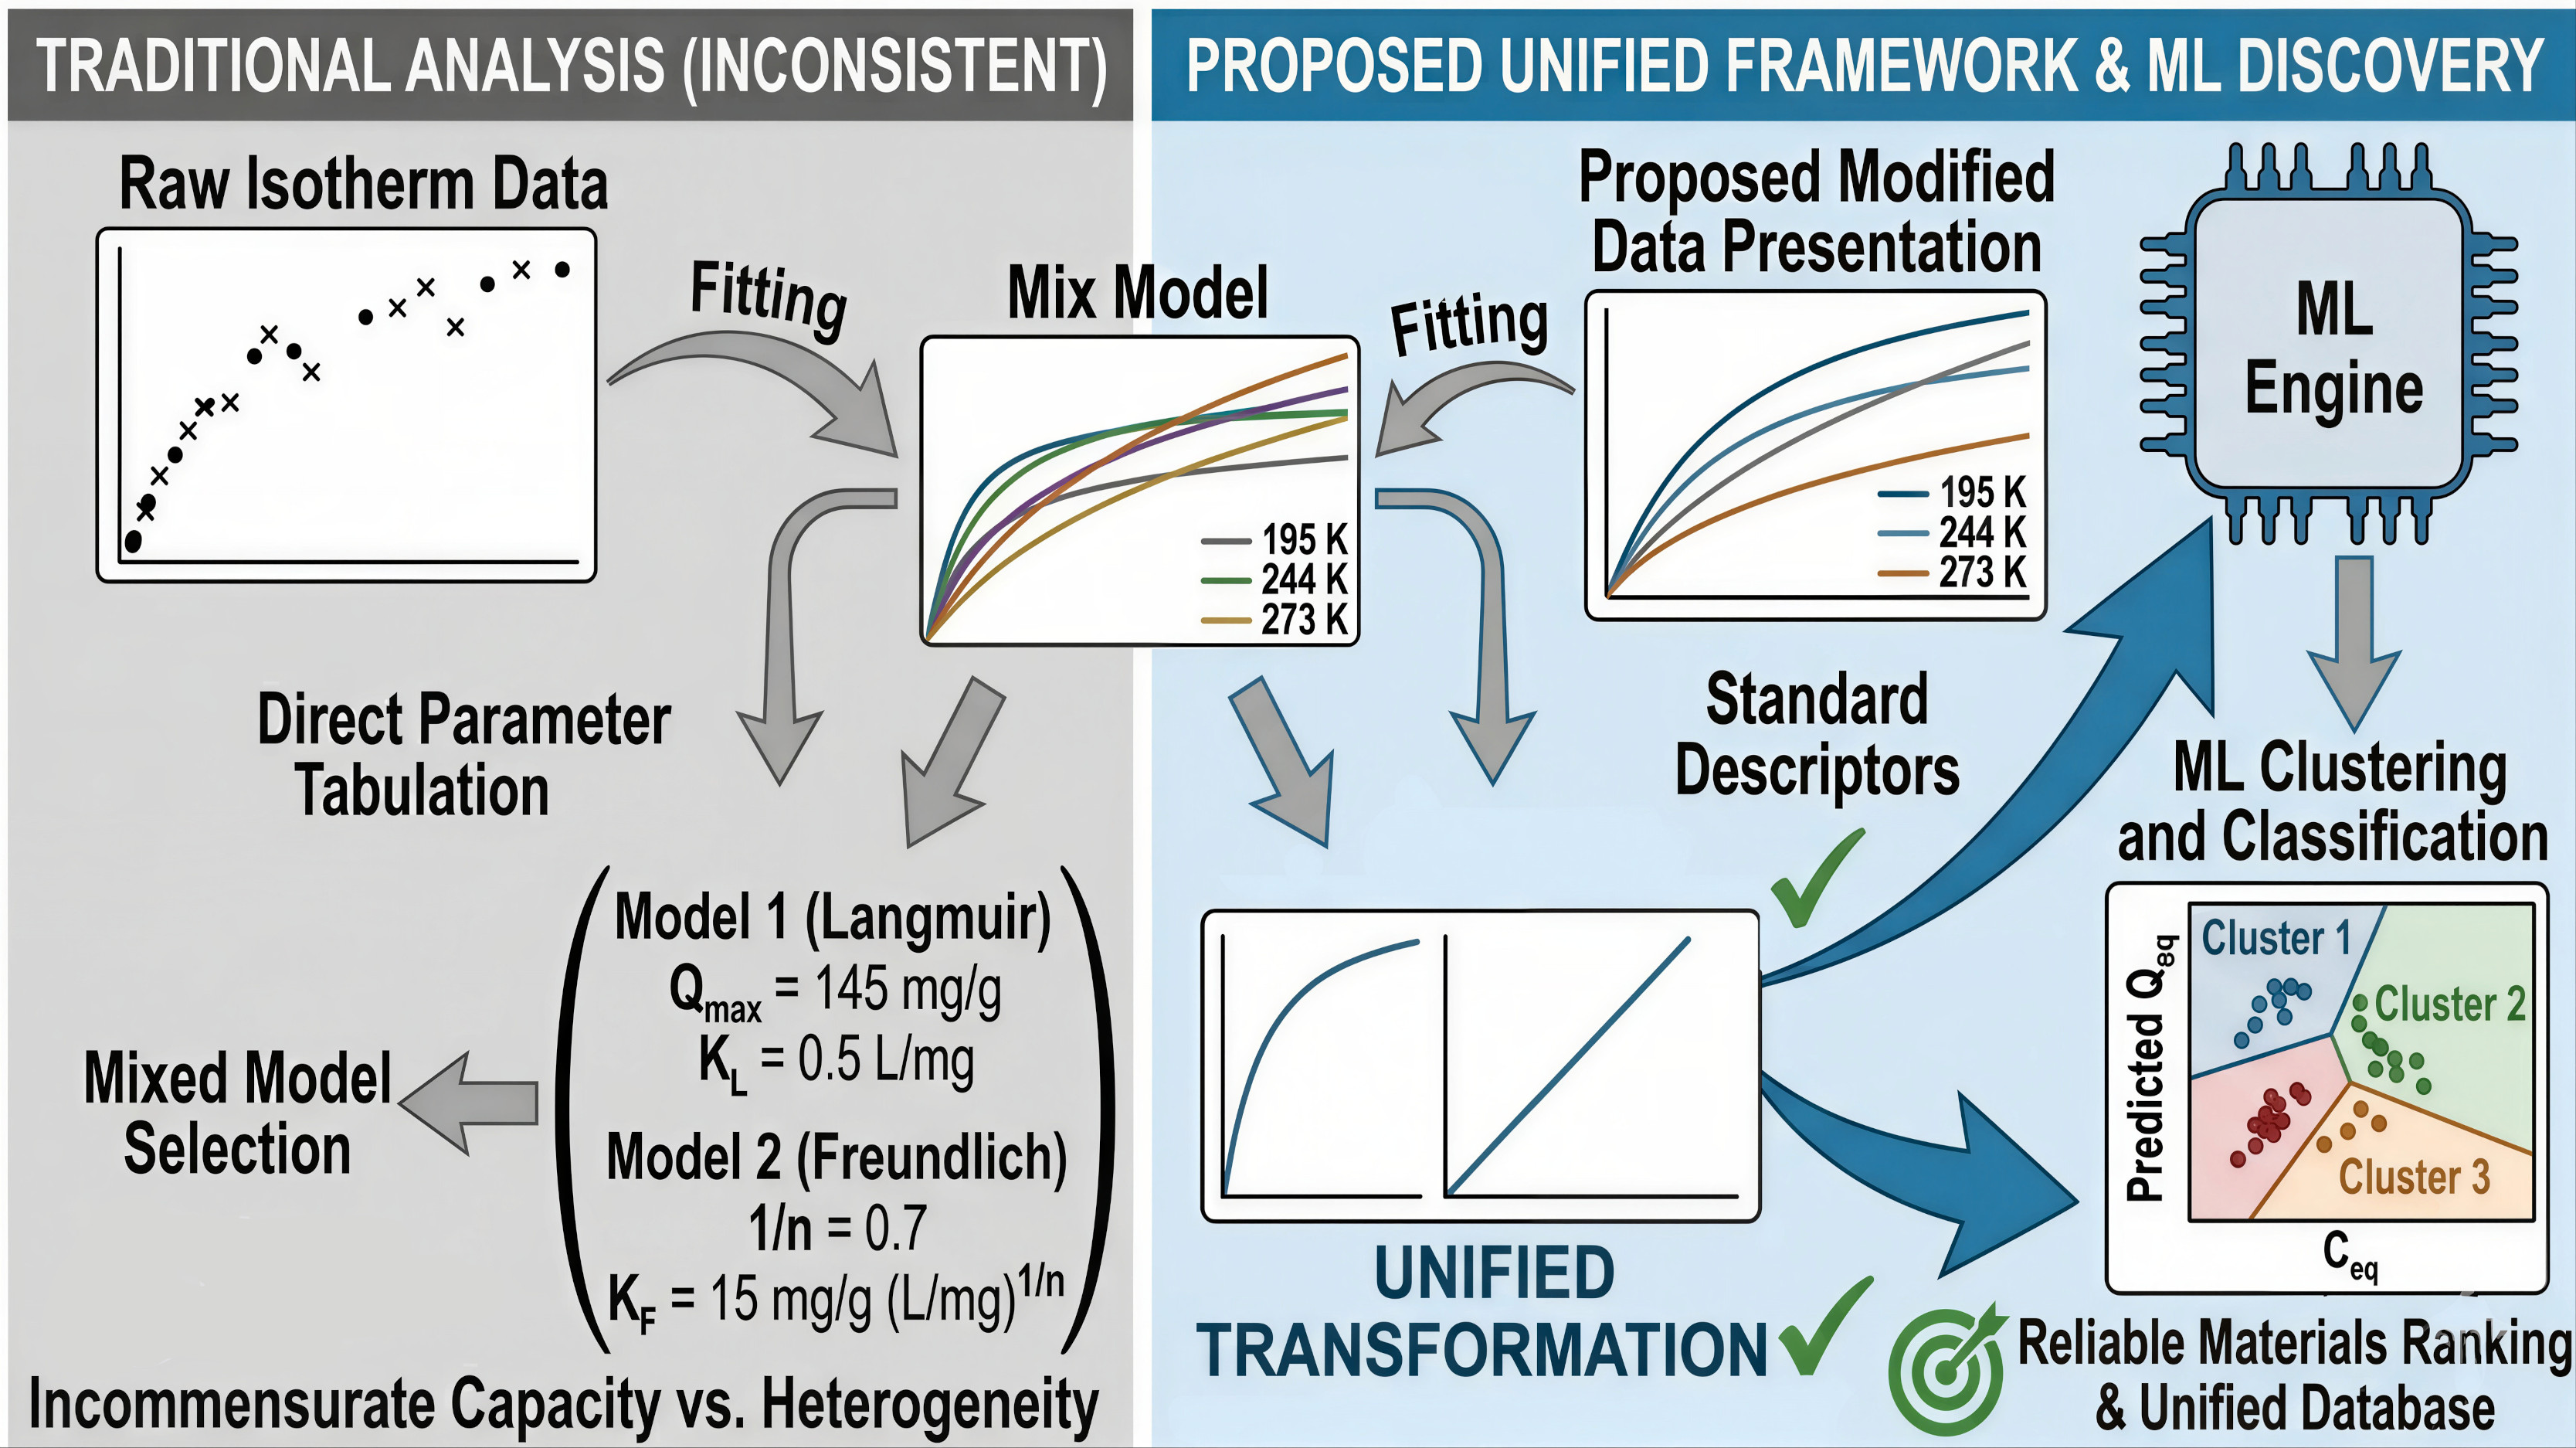
\includegraphics[width=8.1cm]{TOC_Isotherm_LE_upscale_prime_x4_scaled.jpg}
		
		
		% Some journals require a graphical entry for the Table of Contents.
		% This should be laid out ``print ready'' so that the sizing of the
		% text is correct.
		
		% Inside the \texttt{tocentry} environment, the font used is Helvetica
		% 8\,pt, as required by \emph{Journal of the American Chemical
		% 	Society}.
		
		% The surrounding frame is 9\,cm by 3.5\,cm, which is the maximum
		% permitted for  \emph{Journal of the American Chemical Society}
		% graphical table of content entries. The box will not resize if the
		% content is too big: instead it will overflow the edge of the box.
		
		% This box and the associated title will always be printed on a
		% separate page at the end of the document.
		
	\end{tocentry}
	
	%%%%%%%%%%%%%%%%%%%%%%%%%%%%%%%%%%%%%%%%%%%%%%%%%%%%%%%%%%%%%%%%%%%%%
	%% The abstract environment will automatically gobble the contents
	%% if an abstract is not used by the target journal.
	%%%%%%%%%%%%%%%%%%%%%%%%%%%%%%%%%%%%%%%%%%%%%%%%%%%%%%%%%%%%%%%%%%%%%
	\begin{abstract}
		This is an example document for the \textsf{achemso} document
		class, intended for submissions to the American Chemical Society
		for publication. The class is based on the standard \LaTeXe\
		\textsf{report} file, and does not seek to reproduce the appearance
		of a published paper.
		
		This is an abstract for the \textsf{achemso} document class
		demonstration document.  An abstract is only allowed for certain
		manuscript types.  The selection of \texttt{journal} and
		\texttt{manuscript} will determine if an abstract is valid.  If
		not, the class will issue an appropriate error.
	\end{abstract}
	
	%%%%%%%%%%%%%%%%%%%%%%%%%%%%%%%%%%%%%%%%%%%%%%%%%%%%%%%%%%%%%%%%%%%%%
	%% Start the main part of the manuscript here.
	%%%%%%%%%%%%%%%%%%%%%%%%%%%%%%%%%%%%%%%%%%%%%%%%%%%%%%%%%%%%%%%%%%%%%
	\section{Introduction}
	Access to safe water is becoming one of the defining challenges of this century. Global population reached approximately 8.2 billion in 2024 and is projected to approach 9.7 billion by 2050.\cite{noauthor_progress_nodate}. Yet, 2.2 billion people still lack safely managed drinking water services.\cite{noauthor_united_nodate01}. In addition, roughly half of the world's population experiences severe water scarcity for at least part of the year.\cite{mekonnen_four_2016}. Urbanization, industrial activity, agricultural intensification, and climate change are compounding these pressures on global water systems.\cite{vorosmarty_global_2010}. Within this context, the United Nations Sustainable Development Goal~6 (SDG~6), ``Clean Water and Sanitation,'' has catalyzed broad scientific and policy interest in water treatment technologies. However, recent global assessments indicate that the world is not on track to achieve SDG~6 by 2030.\cite{noauthor_blueprint_nodate}
	
	Among the available remediation strategies, adsorption remains especially attractive because of its operational simplicity, compatibility with decentralized treatment, and applicability across a wide range of contaminant classes. Historically, adsorption research in water purification has focused on metals, metalloids, dyes, and pesticides\cite{crini_non-conventional_2006, fu_removal_2011, ahmaruzzaman_industrial_2011}. The contaminant landscape, however, is expanding rapidly and now extends far beyond these classical targets. Contemporary challenges increasingly involve persistent and mobile organic pollutants, pharmaceutical residues, endocrine-disrupting compounds, microplastic-associated chemicals, and, most prominently, per- and polyfluoroalkyl substances (PFAS)\cite{aus_der_beek_pharmaceuticals_2016,thacharodi_water_2023, li_microplastics_2018, rahman_behaviour_2014}. PFAS have become emblematic of the next generation of adsorption targets: they are highly persistent, often mobile in water, resistant to conventional degradation, and subject to tightening regulatory limits in drinking water worldwide\cite{buck_perfluoroalkyl_2011, gluge_overview_2020, us_epa_pfas_2021}. As the diversity of target contaminants grows, so does the need for rigorous, cross-pollutant comparison of adsorbent performance, a task that demands a common descriptive language for adsorption data\cite{foo_insights_2010, hu_critical_2023}.

	Adsorption isotherms are the standard tool for summarizing material performance and for extracting descriptors such as maximum uptake capacity, affinity, and site heterogeneity. In practice, however, parameters obtained from different isotherm models are routinely tabulated side by side as though they were interchangeable. They are not. The Langmuir, double Langmuir, Freundlich, and Sips equations arise from different physical assumptions and assign different meanings, dimensions, and asymptotic behaviors to their fitted constants.\cite{langmuir_adsorption_1918,freundlich_uber_1907,sips_structure_1948} Comparing a Langmuir $Q_\mathrm{max}$ with a value extrapolated from a Freundlich fit, or placing a Langmuir affinity constant next to a Sips affinity constant whose units depend on the heterogeneity exponent, is neither mathematically consistent nor physically meaningful.\cite{latour_langmuir_2015,de_vargas_briao_sips_2023} What often appears to be a comparison of materials is, in reality, a comparison of incompatible parameterizations.\cite{foo_insights_2010}

	This problem is not merely academic. As adsorption studies move toward application-driven screening of advanced sorbents for complex water matrices---including PFAS, pharmaceuticals, and other emerging contaminants---materials are increasingly ranked as ``better'' on the basis of larger fitted constants derived from different models, concentration scales, and assumptions about site heterogeneity. Such practice weakens reproducibility, complicates translation from laboratory results to engineering design, and, most importantly, prevents the community from building reliable structure--performance relationships across adsorbents and pollutants. A field that aims to address global water challenges, including those highlighted by SDG~6 and the rapidly evolving contaminant landscape, requires reporting standards that make adsorption parameters comparable in a thermodynamically meaningful way.
	

	In this work, we propose a practical set of reporting guidelines grounded in the following principles principles. First, capacity comparisons should be restricted to isotherm models for which a finite saturation is explicitly defined---that is, models with a well-defined $Q_\mathrm{max}$, such as Langmuir, double Langmuir, or other saturating forms---while the Freundlich equation should be recognized as unsuitable for reporting a maximum capacity. A full explanation of the availables isotherms is included in the SI.
	Second, raw affinity constants should be replaced, wherever possible, by a standard-state adsorption energy, $E_\mathrm{ads}$, derived from a dimensionless equilibrium constant obtained by normalizing the fitted affinity term with a reference concentration $C^{0}$. This recasts adsorption affinity in a common thermodynamic framework and removes the ambiguity of model-dependent, and sometimes fractional, units. Our broader objective is not to eliminate empirical fitting but to separate the \emph{descriptive} role of an isotherm equation from the \emph{comparative} role of the reported parameters. 
	Third, an statistical guideline to evaluate errors far from the simple and well known R$^2$. This section also incorporates a decision chart to guide the user of this method in chosing the best model to fit their experimental data.
	Forth, a simple Machine learning explanation using k-Nearest Neighbors (KNN) and Support-Vector Machines (SVM) to clusterize materials according to their performance.
	All this information is introduced into three stages, introduction and explanation in the main body, mathematical fundamental in the SI and a series of notebooks with dummy data sets to familiarize the user with the use and another set to fit and evaluate their own data.
	By advocating saturating models for capacity and standard-state energies for affinity, we aim to provide a common language for adsorption reporting---one that is essential if adsorption science is to support credible material screening, reliable benchmarking, and the rational development of sorbents for present and future water-treatment challenges.
	
	% =================================================================
	%  SECTION 2 — THE PROBLEM: INCOMPATIBLE ISOTHERM PARAMETERS
	% =================================================================
	\section{The problem: incompatibility of isotherm-derived parameters}
	\label{sec:problem}

	% --- 2.1  Isotherm models at a glance ---
	\subsection{Common isotherm models and their assumptions}
	\label{sec:models}

	The most widely used isotherm equations in aqueous-phase adsorption can be written as follows. A complete list is included in  \Cref{tab:isotherm_availability} and SI.

\paragraph{Langmuir.}
Assumes a homogeneous surface with a single class of equivalent sites and monolayer coverage:
\begin{equation}
	q_e = \frac{Q_{\max}\, K_L\, C_e}{1 + K_L\, C_e}.
	\label{eq:langmuir}
\end{equation}
Parameters: $Q_{\max}$ (mg.g$^{-1}$), the finite saturation capacity, and $K_L$ (L.mg$^{-1}$), the affinity constant.
See Eq.~\eqref{SI-eq:si_langmuir}.

\paragraph{Double Langmuir.}
Extends Langmuir to two independent site populations:
\begin{equation}
	q_e = \frac{Q_1\, K_1\, C_e}{1 + K_1\, C_e}
	    + \frac{Q_2\, K_2\, C_e}{1 + K_2\, C_e}.
	\label{eq:double_langmuir}
\end{equation}
Total capacity $Q_{\max} = Q_1 + Q_2$ remains finite and well defined.
See Eq.~\eqref{SI-eq:si_double_langmuir}.

\paragraph{Freundlich.}
An empirical power law that describes heterogeneous adsorption without a saturation plateau:
\begin{equation}
	q_e = K_F\, C_e^{1/n}.
	\label{eq:freundlich}
\end{equation}
$K_F$ has concentration-dependent units (mg.g$^{-1}$)(L.gg$^{-1}$)$^{1/n}$; no $Q_{\max}$ is defined.
See Eq.~\eqref{SI-eq:si_freundlich}.

	\paragraph{Sips (Langmuir--Freundlich).}
	Introduces surface heterogeneity through an exponent $m$ while retaining a saturation plateau:
	\begin{equation}
		q_e = \frac{Q_{\max}\,(K_S\, C_e)^{m}}{1 + (K_S\, C_e)^{m}}.
		\label{eq:sips}
	\end{equation}
	When $m = 1$, Sips reduces to Langmuir. The affinity constant $K_S$ carries units that depend on $m$, i.e.\ (L.mg$^{-1}$)$^{m}$, and is therefore not directly comparable with $K_L$.
	See Eq.~\eqref{SI-eq:si_sips}.
	
	As shown in Figure~\ref{fig:isotherm_model_selection_workflow}, the model selection procedure combines physical screening, statistical comparison, and physicochemical validation.
	
	\newpage

	\begin{table}[H]
		\small
		\caption{Availability of $Q_{\max}$, $K_H$, and an effective affinity constant $K_{\mathrm{aff}}$ for common isotherm models, together with their implied energy-distribution family. The ``Recommended use'' column is \textcolor{green!50!black}{YES} when both $Q_{\max}$ and a comparable $K_{\mathrm{aff}}$ can be reported, and \textcolor{red}{NO} otherwise. See the SI sections in the last column for the derivations and definitions.}
		\label{tab:isotherm_availability}
		\renewcommand{\arraystretch}{1.2}
		\begin{tabular}{@{} p{2.0cm} p{1.0cm} c c p{3.0cm} p{3.8cm} p{1.8cm} @{}}
			\hline
			\textbf{Model}
			& $\boldsymbol{Q_{\max}}$
			& $\boldsymbol{K_H}$
			& $\boldsymbol{K_{\mathrm{aff}}}$
			& \textbf{Recommended}
			& \textbf{Energy distribution}
			& \textbf{SI ref.} \\
			\hline
			Henry
			& \textcolor{red}{No} & \textcolor{green!50!black}{Yes} & \textcolor{red}{No}
			& \textcolor{red}{NO}
			& -- (low-coverage limit)
			& \ref{SI-sec:si_henry} \\
			Langmuir
			& \textcolor{green!50!black}{Yes} & \textcolor{green!50!black}{Yes} & \textcolor{green!50!black}{Yes}
			& \textcolor{green!50!black}{YES}
			& Dirac $\delta$
			& \ref{SI-sec:si_langmuir} \\
			Double Langmuir
			& \textcolor{green!50!black}{Yes} & \textcolor{green!50!black}{Yes} & \textcolor{green!50!black}{Yes}
			& \textcolor{green!50!black}{YES}
			& Two Dirac $\delta$
			& \ref{SI-sec:si_double_langmuir} \\
			Freundlich
			& \textcolor{red}{No} & \textcolor{orange!80!black}{Cond.} & \textcolor{red}{No}
			& \textcolor{red}{NO}
			& Power law %(unbounded)
			& \ref{SI-sec:si_freundlich} \\
			Sips (L--F)
			& \textcolor{green!50!black}{Yes} & \textcolor{orange!80!black}{Cond.} & \textcolor{green!50!black}{Yes} $^*$
			& \textcolor{green!50!black}{YES}
			& Logistic
			& \ref{SI-sec:si_sips} \\
			T\'{o}th
			& \textcolor{green!50!black}{Yes} & \textcolor{green!50!black}{Yes} & \textcolor{green!50!black}{Yes}
			& \textcolor{green!50!black}{YES}
			& Gen.\ logistic (asym.)
			& \ref{SI-sec:si_toth} \\
			Jovanovic
			& \textcolor{green!50!black}{Yes} & \textcolor{green!50!black}{Yes} & \textcolor{green!50!black}{Yes}
			& \textcolor{green!50!black}{YES}
			& Gumbel (EV-I)
			& \ref{SI-sec:si_jovanovic} \\
			Temkin
			& \textcolor{red}{No} & \textcolor{red}{No} & \textcolor{green!50!black}{Yes} $^*$
			& \textcolor{red}{NO}
			& Uniform (rect.)
			& \ref{SI-sec:si_temkin} \\
			UNILAN
			& \textcolor{green!50!black}{Yes} & \textcolor{green!50!black}{Yes} $^*$ & \textcolor{green!50!black}{Yes}
			& \textcolor{green!50!black}{YES}
			& Uniform (rect.)
			& \ref{SI-sec:si_unilan} \\
			Redlich--Peterson
			& \textcolor{orange!80!black}{Cond.} & \textcolor{green!50!black}{Yes} & \textcolor{green!50!black}{Yes} $^*$
			& \textcolor{red}{NO}
			& Non-standard (asym.)
			& \ref{SI-sec:si_redlich_peterson} \\
			Koble--Corrigan
			& \textcolor{green!50!black}{Yes} & \textcolor{orange!80!black}{Cond.} & \textcolor{green!50!black}{Yes} $^*$
			& \textcolor{green!50!black}{YES}
			& Logistic (Sips  like)
			& \ref{SI-sec:si_koble_corrigan} \\
			Radke--Prausnitz
			& \textcolor{red}{No} & \textcolor{green!50!black}{Yes} & \textcolor{orange!80!black}{Cond.} $^*$
			& \textcolor{red}{NO}
			& Non-standard (asym.)
			& \ref{SI-sec:si_radke_prausnitz} \\
			D-R / D-A
			& \textcolor{green!50!black}{Yes} & \textcolor{red}{No} & \textcolor{green!50!black}{Yes} $^*$
			& \textcolor{green!50!black}{YES}
			& Rayleigh / Weibull
			& \ref{SI-sec:si_dr_da} \\
			Hill
			& \textcolor{green!50!black}{Yes} & \textcolor{orange!80!black}{Cond.} & \textcolor{green!50!black}{Yes} $^*$
			& \textcolor{green!50!black}{YES}
			& Logistic (Sips like)
			& \ref{SI-sec:si_hill} \\
			\hline
		\end{tabular}
	\end{table}

	\noindent\textbf{Notes.} ``Cond.'' indicates availability only in special parameter limits (e.g., $m=1$, $n_H=1$, $\beta=1$). ``$^*$.'' indicates an effective or operational definition; see the SI for explicit formulas and limits.
	
	
	\begin{figure}[H]
		\centering
		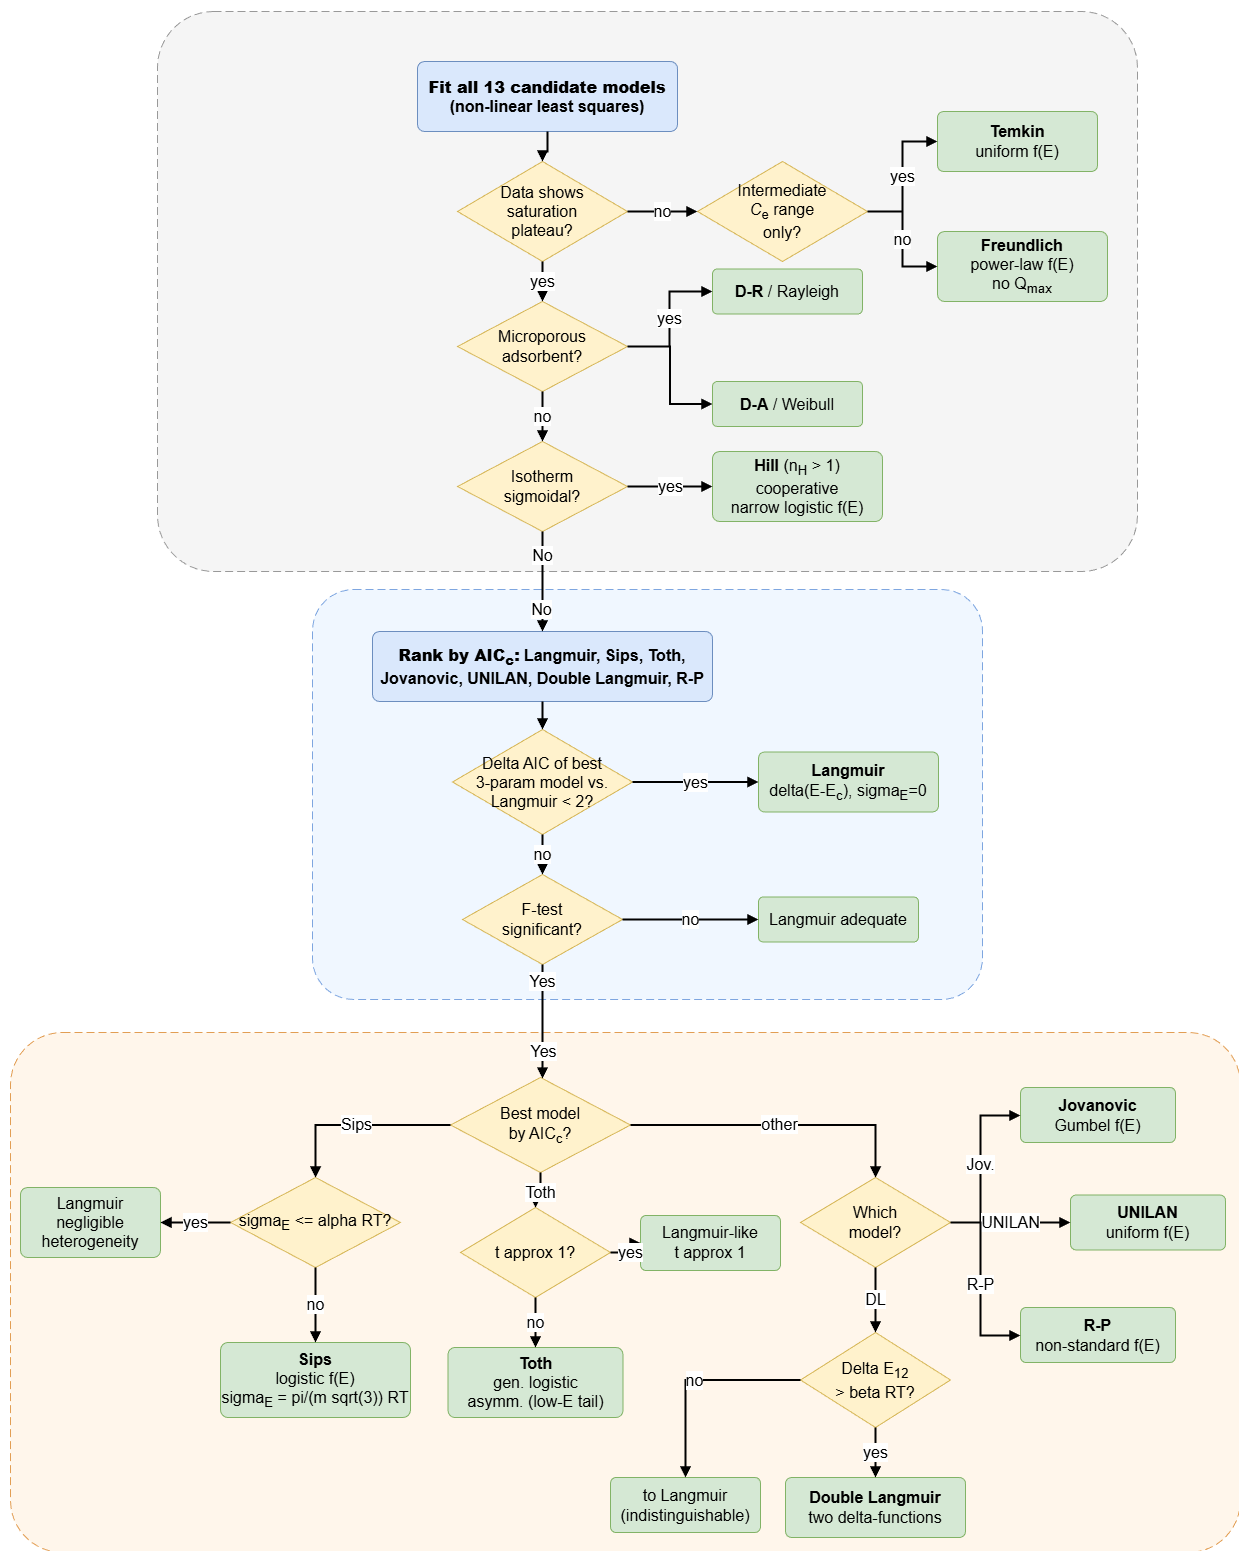
\includegraphics[width=\columnwidth]{Isotherms.drawio_crop.png}
	\caption{Workflow for adsorption isotherm model selection combining shape-based screening, AIC/F-test ranking, and physical validation via heterogeneity and energy distributions.}
		\label{fig:isotherm_model_selection_workflow}
	\end{figure}
	
	

	% --- 2.2  Why Qmax values are not comparable ---
\subsection{Why $Q_{\max}$ values are not always comparable}
\label{sec:qmax_problem}

%TODO: Prose explaining:
% - Langmuir and Double Langmuir define Qmax explicitly (finite plateau)
	% - Freundlich has NO Qmax — it diverges as Ce → ∞
	% - Some authors "extract" Qmax from Freundlich by evaluating at an
	%   arbitrary Ce, but this is physically meaningless
	% - Sips defines Qmax, but if m deviates strongly from 1 the plateau
	%   may lie far outside the experimental concentration window
% - Consequence: tables that mix Langmuir-Qmax with Freundlich-derived
%   values are comparing fundamentally different quantities

Even though $Q_{\max}$ is often treated as a universal figure of merit, it is
model-specific unless the isotherm explicitly contains a finite saturation
plateau. In the Langmuir and Double Langmuir equations, $Q_{\max}$ (or
$Q_1 + Q_2$) is a true asymptote: it is the coverage reached as $C_e \to \infty$
and is therefore a well-defined thermodynamic capacity. By contrast, the
Freundlich isotherm has no saturation term; $q_e$ increases without bound as
$C_e$ increases (SI Eq.~\eqref{SI-eq:si_freundlich}), so any ``$Q_{\max}$''
inferred from a Freundlich fit depends
entirely on the chosen concentration window. Reporting such a value as a
capacity is physically meaningless because it is not a model parameter and has
no invariant interpretation.

%Even for models that do saturate, comparability depends on where the plateau falls relative to the experimental data. In the Sips equation, for example, the heterogeneity exponent $m$ can shift the approach to saturation far outside the measured range (See Eq.~\ref{SI-eq:si_sips}). A fitted $Q_{\max}$ then becomes an extrapolation rather than a  data-supported capacity. The practical consequence is that tables mixing Langmuir or Double Langmuir $Q_{\max}$ values with Freundlich-derived or far-extrapolated capacities are not comparing the same physical quantity. Any ranking built on such a mixture conflates true saturation capacities with model-dependent extrapolations.

Even for models that do saturate, comparability depends on whether the saturation regime is actually constrained by the experimental data. In the Sips equation, for example, the heterogeneity exponent $m$ can shift the onset of saturation far beyond the measured concentration range (see Eq.~\ref{SI-eq:si_sips}). Under these conditions, the fitted $Q_{\max}$ is not determined by the data but inferred through extrapolation. As a result, reported capacities may reflect model-imposed asymptotes rather than experimentally supported saturation values. The practical consequence is that tables mixing Langmuir or Double Langmuir $Q_{\max}$ values with Freundlich-derived or poorly constrained Sips capacities are not comparing the same physical quantity. Any ranking built on such a mixture conflates experimentally supported saturation capacities with model-dependent extrapolations.

	% --- 2.3  Why Kaff values are not comparable ---
\subsection{Why affinity constants are not comparable across models}
\label{sec:kaff_problem}

%TODO: Prose explaining:
% - KL (Langmuir) has units L/mg — a reciprocal concentration
	% - KS (Sips) has units (L/mg)^m — fractional, model-dependent
	% - KF (Freundlich) has mixed units that depend on 1/n
	% - KH (Henry constant) is a low-coverage slope, not a full-isotherm descriptor
% - Even when symbols look similar, the numbers are incommensurate
% - Placing KL next to KS in a table is comparing apples to oranges

Affinity constants carry the strongest illusion of comparability because they
are reported as single numbers, yet their physical meaning and units change
from model to model. In the Langmuir equation, $K_L$ has units of inverse
concentration (e.g., L.mg$^{-1}$) and sets the midpoint of the uptake curve.
In the Sips equation, the constant $K_S$ carries units of
(L.mg$^{-1}$)$^{m}$, which depend on the heterogeneity exponent $m$; therefore
its numerical value is not on the same scale as $K_L$ unless $m = 1$
(SI Eqs.~\eqref{SI-eq:si_langmuir} and \eqref{SI-eq:si_sips}). The Freundlich
constant $K_F$ is even less comparable, because its units depend on $1/n$ and it
does not correspond to any saturation behavior (SI
Eq.~\eqref{SI-eq:si_freundlich}).

The Henry constant $K_H$ provides a low-coverage slope (SI
Eq.~\eqref{SI-eq:si_henry}), but it is not a
full-isotherm descriptor and cannot replace affinity constants derived from
different functional forms without additional normalization. As a result,
placing $K_L$, $K_S$, and $K_F$ side by side implies a common meaning that does
not exist. Any comparison based on raw affinity constants is therefore a
comparison of incommensurate parameters, not of intrinsic adsorption strength.

	% =================================================================
	%  SECTION 3 — THE PROPOSAL: STANDARD-STATE ADSORPTION ENERGY
	% =================================================================
	\section{A common language: standard-state adsorption energy}
	\label{sec:proposal}

	% --- 3.1  Dimensionless equilibrium constant ---
	\subsection{Constructing a dimensionless equilibrium constant}
	\label{sec:dimensionless_K}

	To place all isotherm models on a common footing, the model-specific affinity constant is converted into a dimensionless quantity by referencing it to a declared standard-state concentration $C^{0}$:
	\begin{equation}
		K_{\mathrm{aff}}^{\ast}
		= \frac{K_H}{Q_{\max}}\; C^{0},
		\label{eq:Kaff_star}
	\end{equation}
	where $K_H = \lim_{C_e \to 0} (q_e / C_e)$ is the Henry constant (initial slope of the isotherm). Because $K_H / Q_{\max}$ has units of inverse concentration, multiplication by $C^{0}$ renders $K_{\mathrm{aff}}^{\ast}$ dimensionless regardless of the isotherm model from which $K_H$ is extracted.

	% --- 3.2  Standard-state adsorption energy ---
	\subsection{Standard-state adsorption energy $E_{\mathrm{ads}}$}
	\label{sec:Eads}

	The standard-state adsorption energy is obtained directly from the dimensionless equilibrium constant:
	\begin{equation}
		E_{\mathrm{ads}} = RT \ln K_{\mathrm{aff}}^{\ast}.
		\label{eq:Eads}
	\end{equation}
	This quantity has units of kJ.mol$^{-1}$, is independent of the isotherm model used, and provides a thermodynamically meaningful measure of affinity that can be compared across adsorbents, contaminants, and laboratories.

	% --- 3.3  Extraction from each model ---
	\subsection{Extraction of $K_{\mathrm{aff}}^{\ast}$ and $E_{\mathrm{ads}}$ from each model}
	\label{sec:extraction}

	Table~\ref{tab:extraction} shows how $K_{\mathrm{aff}}^{\ast}$ and $E_{\mathrm{ads}}$ are obtained from the native parameters of each isotherm.

	\begin{table}[H]
		\small
		\caption{Extraction of universal descriptors from native isotherm parameters. $C^{0}$ is the declared standard-state concentration.}
		\label{tab:extraction}
		\renewcommand{\arraystretch}{1.3}
		\begin{tabular}{@{} l c c c @{}}
			\hline
			\textbf{Model}
			& $\boldsymbol{Q_{\max}}$
			& $\boldsymbol{K_{\mathrm{aff}}}$ \textbf{(native)}
			% & $\boldsymbol{K_{\mathrm{aff}}^{\ast}}$ \textbf{(dimless)}
			& $\boldsymbol{E_{\mathrm{ads}}/(RT)}$ \\
			\hline
			Langmuir
			& $Q_{\max}$
			& $K_L$
			% & $K_L\, C^{0}$
			& $\ln(K_L\, C^{0})$ \\
			Double Langmuir
			& $Q_1 + Q_2$
			& $K_L^{\mathrm{(tot)}} = \dfrac{Q_1K_1 + Q_2K_2}{Q_1+Q_2}$
			& $\ln(K_L^{\mathrm{(tot)}}\, C^{0})$ \\
			Sips
			& $Q_{\max}$
			& $K_S^{1/m}$
			% & $(K_S)^{1/m}\, C^{0}$
			& $\frac{1}{m}\ln(K_S\, (C^{0})^{m})$ \\
			T\'{o}th
			& $q_{\max}$
			& $b$
			% & $b\, C^{0}$
			& $\ln(b\, C^{0})$ \\
			Jovanovic
			& $q_{\max}$
			& $b$
			% & $b\, C^{0}$
			& $\ln(b\, C^{0})$ \\
			Temkin
			& ---
			& $a_T$
			% & $a_T\, C^{0}$
			& $\ln(a_T\, C^{0})$ \\
			UNILAN
			& $Q_{\max}$
			& $\sqrt{b_{\max} b_{\min}}$
			% & $\sqrt{b_{\max} b_{\min}}\; C^{0}$
			& $\tfrac{1}{2}\ln(b_{\max} b_{\min}\,(C^{0})^{2})$ \\
			Redlich--Peterson
			& $K_{RP}/a_{RP}$\,$^{a}$
			& $a_{RP}$\,$^{a}$
			% & $a_{RP}\, C^{0}$
			& $\ln(a_{RP}\, C^{0})$ \\
			Koble--Corrigan
			& $A_{KC}/B_{KC}$
			& $B_{KC}^{\,n}$
			% & $B_{KC}^{\,n}\, C^{0}$
			& $n\ln(B_{KC}\, C^{0})$ \\
			Radke--Prausnitz
			& ---
			& $r_{RP}$
			% & $r_{RP}\, C^{0}$
			& $\ln(r_{RP}\, C^{0})$ \\
			D-R / D-A
			& $Q_{\max}$
			& $1/C_{1/2}$\,$^{b}$
			% & $C^{0}/C_{1/2}$
			& $\ln(C^{0}/C_{1/2})$ \\
			Hill
			& $Q_{\max}$
			& $K_D^{-1/n_H}$
			% & $K_D^{-1/n_H}\, C^{0}$
			& $-\frac{1}{n_H}\ln K_D + \ln C^{0}$ \\
			\hline
		\end{tabular}

		\smallskip
		\noindent $^{a}$\,Only when $\beta = 1$.\quad
		$^{b}$\,$C_{1/2}$ is the half-loading concentration; see Sec.~\ref{SI-sec:si_dr_da}.\quad
		``---'' indicates no finite $Q_{\max}$ exists.
	\end{table}

	The Freundlich isotherm is deliberately absent from Table~\ref{tab:extraction}: because it defines no finite $Q_{\max}$, the ratio $K_H/Q_{\max}$ is undefined and no dimensionless affinity can be constructed. For the Double Langmuir model, an effective total adsorption energy can be reported from the capacity-weighted constant $K_L^{\mathrm{(tot)}}$, while the site-resolved constants $K_1$ and $K_2$ remain necessary to preserve the bimodal interpretation captured by the site separation descriptor. Finally, the choice of standard-state concentration $C^{0}$ must be explicitly declared; although it appears inside the logarithm and therefore cancels in any \emph{difference} $\Delta E_{\mathrm{ads}}$, it must be consistent across all entries in a comparative table. The full set of energy-distribution families and their relation to $\sigma_H$ is given in Table~\ref{SI-tab:si_energy_dist_families}; numerical values of $\sigma_H$ at $T = 298$~K are collected in Table~\ref{SI-tab:si_sigma_numerical}.

\begin{comment}


	% =================================================================
	%  SECTION 4 — HETEROGENEITY: THE ENERGY DISTRIBUTION
	% =================================================================
	\section{Quantifying surface heterogeneity: energy distributions}
	\label{sec:heterogeneity}

	% --- 4.1  The condensation approximation ---
	\subsection{From isotherms to energy distributions}
	\label{sec:condensation}

	The final variable in the system is the distribution of adsorption site energies, which is typically neither explicitly reported nor directly fitted. However, each isotherm model implies a characteristic site-energy distribution (see \Cref{tab:energy_distributions}).

	Real adsorbent surfaces are energetically heterogeneous because adsorption sites differ in local chemistry, accessible geometry, and coordination environment. As a result, adsorption is better described by a distribution of site energies than by a single adsorption energy. A heterogeneous surface can therefore be represented as an ensemble of independent Langmuir-type sites with adsorption energy $E$, and the macroscopic isotherm is obtained by integrating the local occupancy over the site-energy distribution $f(E)$:
	\begin{equation}
		q_e = Q_{\max} \int_{0}^{\infty}
		\frac{K(E)\, C_e}{1 + K(E)\, C_e}\; f(E)\, \mathrm{d}E,
		\label{eq:heterogeneous_integral}
	\end{equation}
	where $K(E) = K_0 \exp(E/RT)$ is the local Langmuir affinity at energy~$E$ and $f(E)$ is normalised to unity. Each choice of $f(E)$ generates a different macroscopic isotherm; conversely, each isotherm model implies a specific functional form for $f(E)$.

	The \emph{condensation approximation} provides a practical route from any empirical isotherm equation back to the underlying distribution. The Langmuir kernel is replaced by a unit step at the \emph{condensation energy}~$E_c$:
	\begin{equation}
		\frac{K(E)\,C_e}{1+K(E)\,C_e} \;\approx\; \Theta(E - E_c),
		\qquad
		E_c = RT\ln\!\left(\frac{1}{K_0 C_e}\right).
		\label{eq:condensation_step}
	\end{equation}
	Substituting $C_e = C^{\ast}\exp(-E/RT)$ and differentiating yields
	\begin{equation}
		f(E) \;=\; -\frac{1}{Q_{\max}}\frac{\mathrm{d}q}{\mathrm{d}E},
		\label{eq:fE_general}
	\end{equation}
	where $q$ is expressed as a function of $E$ via the substitution above. Full derivations for all isotherm models are collected in Section~\ref{SI-sec:si_individual_distributions}.

	% --- 4.2  Energy-distribution families ---
	\subsection{Energy-distribution families and $\sigma_E$}
	\label{sec:energy_families}

	Applying Eq.~\eqref{eq:fE_general} to each isotherm yields the energy-distribution families summarised in Table~\ref{tab:energy_distributions}.

	\begin{table}[H]
		\small
		\caption{Energy-distribution families and intrinsic heterogeneity width $\sigma_H$ implied by each isotherm model. Parameter $m$ (Sips, Koble--Corrigan) is the heterogeneity exponent; $t$ (T\'{o}th) and $n_H$ (Hill) are the respective shape parameters. $\sigma_H$ is in units of $RT$ ($RT\approx 2.48$~kJ\,mol$^{-1}$ at $298$~K). Full derivations: Section~\ref{SI-sec:si_individual_distributions}.}
		\label{tab:energy_distributions}
		\renewcommand{\arraystretch}{1.4}
		\begin{tabular}{@{} l l c l @{}}
			\hline
			\textbf{Model}
			& \textbf{Distribution $f(E)$}
			& \textbf{Symm.}
			& $\boldsymbol{\sigma_H/(RT)}$ \\
			\hline
			Langmuir
			& Dirac $\delta(E-E_c)$
			& ---
			& $0$ \\
			Double Langmuir
			& Two Dirac $\delta$
			& ---
			& $\tfrac{\sqrt{Q_1 Q_2}}{Q_1+Q_2}\tfrac{|\Delta E_{12}|}{RT}$ \\
			Sips
			& Logistic (scale $RT/m$)
			& Yes
			& $\sqrt{1/m^2-1}$ \\
			T\'{o}th
			& Gen.\ logistic type IV
			& No
			& $>\pi/\sqrt{3}$\;$(t<1)$; no closed form \\
			Jovanovic
			& Gumbel (EV-I)
			& No
			& $\pi/\sqrt{6}\approx 1.28$ \\
			Temkin
			& Uniform
			& Yes
			& $b_T Q_{\max}/(2\sqrt{3}\,RT)$ \\
			UNILAN
			& Uniform (exact kernel)
			& Yes
			& $\ln(b_{\max}/b_{\min})/(2\sqrt{3})$ \\
			Freundlich
			& Power law (unbounded)
			& ---
			& $\infty$ \\
			Redlich--Peterson
			& Non-standard ($\beta < 1$)
			& No
			& --- \\
			Koble--Corrigan
			& $\equiv$ Sips
			& Yes
			& $\sqrt{1/m^2-1}$ \\
			Radke--Prausnitz
			& Non-standard
			& No
			& --- \\
			D-R ($n_{DA}=2$)
			& Rayleigh
			& No
			& $0.463\,E_a/(RT)$ \\
			D-A (general)
			& Weibull (shape $n_{DA}$)
			& No
			& $(E_a/RT)\sqrt{\Gamma(1+2/n_{DA})-[\Gamma(1+1/n_{DA})]^2}$ \\
			Hill
			& $\equiv$ Sips (scale $RT/n_H$)
			& Yes
			& $\sqrt{\max(1/n_H^2-1,0)}$ \\
			\hline
		\end{tabular}
	\end{table}

	Several physical patterns emerge from Table~\ref{tab:energy_distributions}:
	\begin{itemize}
		\item \textbf{Homogeneous limit.} The Langmuir model corresponds to a single energy level ($\sigma_E = 0$). Double Langmuir adds a second discrete level; $\sigma_E$ measures the energy separation weighted by the site capacities $Q_1, Q_2$.

		\item \textbf{Symmetric logistic family.} Sips, Koble--Corrigan, and Hill all imply a symmetric logistic distribution. The width $\sigma_E = \pi RT/(m\sqrt{3})$ increases as $m \to 0$ (or $n_H \to 0$), recovering Freundlich-like behaviour in the limit.

		\item \textbf{Asymmetric distributions.} T\'{o}th generates a distribution skewed toward \emph{low}-energy (weak-binding) sites, consistent with its pronounced low-coverage tail. Jovanovic generates a Gumbel distribution skewed toward \emph{high}-energy sites, with a fixed intrinsic width independent of the affinity parameter~$b$.

		\item \textbf{Uniform distributions.} Temkin and UNILAN both assume a flat rectangular energy distribution. UNILAN retains the exact Langmuir integral; Temkin uses the condensation approximation. Their $\sigma_E$ is set entirely by the half-width of the uniform energy band.

		\item \textbf{Divergent and non-analytical cases.} Freundlich has $\sigma_E = \infty$, directly reflecting the absence of~$Q_{\max}$. Redlich--Peterson and Radke--Prausnitz yield empirical distributions without closed-form variances.

		\item \textbf{Dubinin models.} D-R and D-A operate in the Polanyi adsorption potential $\varepsilon = RT\ln(1+1/C_e)$. The distribution in $\varepsilon$ is Weibull; the D-R case ($n_{DA} = 2$) gives the Rayleigh distribution with $\sigma_\varepsilon \approx 0.463\,E_a$.
	\end{itemize}

	% --- 4.3  Physical interpretation of sigma_E ---
	\subsection{Physical interpretation of $\sigma_E$}
	\label{sec:sigma_E}

	The standard deviation $\sigma_E$ of the site-energy distribution is the third universal descriptor. It is derived analytically from the same isotherm parameters as $E_{\mathrm{ads}}$, imposing no additional fitting burden. A small $\sigma_E \ll RT$ indicates a nearly homogeneous surface; $\sigma_E \sim RT$ corresponds to moderate heterogeneity; and $\sigma_H \gg RT$ signals broad energetic diversity typical of activated carbons, biochars, or disordered porous solids. At $T = 298$~K, the intrinsic logistic width (Sips, $m = 1$) is $(\pi/\sqrt{3})\,RT \approx 4.5$~kJ\,mol$^{-1}$; surfaces below this threshold are practically indistinguishable from Langmuir behaviour. Numerical $\sigma_E$ values for representative parameter choices are tabulated in Table~\ref{SI-tab:si_sigma_numerical}.
	
	The usefulness of $\sigma_E$ extends beyond describing surface heterogeneity. Because it is derived from the fitted isotherm parameters on the same footing as $Q_{\max}$ and $E_{\mathrm{ads}}$, it converts model-specific heterogeneity into a common statistical descriptor. This enables comparison of competing models not only through residual-based criteria such as SSE, AIC$_c$, BIC, or F-tests, but also through the physical similarity of their implied site-energy distributions, for example by overlap metrics. More broadly, the descriptor set $\{Q_{\max}, E_{\mathrm{ads}}, \sigma_E\}$ defines a common feature space in which adsorbent--adsorbate systems can be grouped, ranked, or separated using statistical learning tools such as k-Nearest Neighbours (KNN) and Support Vector Machines (SVM). In this way, the site-energy distribution becomes the link between isotherm physics, statistical model comparison, and data-driven classification.

\end{comment}

	% =================================================================
	%  SECTION 4 -- HETEROGENEITY: THE ENERGY DISTRIBUTION
	% =================================================================
	\section{Quantifying surface heterogeneity: energy distributions}
	\label{sec:heterogeneity}
	
	% --- 4.1  From site energies to observable isotherms ---
	\subsection{From adsorption sites to observable energy distributions}
	\label{sec:condensation}
	
	The final variable in the adsorption system is the distribution of site energies. Unlike $Q_{\max}$ or $E_{\mathrm{ads}}$, this quantity is usually not fitted explicitly, yet it is implicitly encoded in every isotherm model. In other words, each adsorption equation corresponds to a particular assumption about how adsorption energies are distributed across the surface. This provides a natural way to place different isotherm models in a common physical framework.
	
	Real adsorbent surfaces are energetically heterogeneous because adsorption sites differ in local chemistry, accessible geometry, coordination environment, and confinement. As a result, adsorption is more realistically described by a distribution of site energies than by a single characteristic value. A heterogeneous surface can therefore be represented as an ensemble of independent Langmuir-type sites, each characterized by an adsorption energy $E$, so that the macroscopic isotherm is written as
	\begin{equation}
		q_e
		=
		Q_{\max}
		\int_{-\infty}^{\infty}
		\Theta_L(E-E_c)\, f(E)\,\mathrm{d}E,
		\label{eq:heterogeneous_integral}
	\end{equation}
	where $f(E)$ is the normalized distribution of adsorption site energies,
	\begin{equation}
		\int_{-\infty}^{\infty} f(E)\,\mathrm{d}E = 1,
	\end{equation}
	and $\Theta_L(E-E_c)$ is the Langmuir occupation kernel,
	\begin{equation}
		\Theta_L(E-E_c)
		=
		\frac{1}{1+\exp\!\left[-(E-E_c)/(RT)\right]}.
		\label{eq:langmuir_kernel_energy}
	\end{equation}
	Here $E_c$ is the condensation energy associated with the equilibrium concentration,
	\begin{equation}
		E_c = RT\ln\!\left(\frac{1}{K_0 C_e}\right),
		\label{eq:condensation_energy}
	\end{equation}
	with $K_0$ a reference constant used to define the energy scale.
	
	Equation~\eqref{eq:heterogeneous_integral} emphasizes an important point: the experimentally observed isotherm does not probe the intrinsic distribution $f(E)$ directly, but rather the convolution of that distribution with the thermal occupation kernel. Differentiating eq~\eqref{eq:heterogeneous_integral} with respect to $E_c$ gives the observable energy-density profile
	\begin{equation}
		\phi(E_c)
		=
		-\frac{1}{Q_{\max}}\frac{\mathrm{d}q_e}{\mathrm{d}E_c}
		=
		\int_{-\infty}^{\infty}
		f(E)\, g_T(E-E_c)\,\mathrm{d}E,
		\label{eq:observable_distribution}
	\end{equation}
	where
	\begin{equation}
		g_T(x)
		=
		\frac{\exp(-x/RT)}
		{RT\left[1+\exp(-x/RT)\right]^2}
		\label{eq:thermal_kernel}
	\end{equation}
	is the thermal broadening kernel. This kernel is a logistic probability density with standard deviation
	\begin{equation}
		\sigma_T = \frac{\pi}{\sqrt{3}}RT.
		\label{eq:thermal_sigma}
	\end{equation}
	
	Thus, even a perfectly homogeneous Langmuir surface, intrinsically described by a Dirac distribution,
	\begin{equation}
		f(E) = \delta(E-E_1),
		\label{eq:delta_langmuir}
	\end{equation}
	is observed through the broadened profile
	\begin{equation}
		\phi(E_c) = g_T(E_1-E_c),
		\label{eq:single_site_broadened}
	\end{equation}
	which already has a finite width set by temperature. At $T=298$~K, this intrinsic thermal width is
	\begin{equation}
		\sigma_T \approx 4.5~\mathrm{kJ\,mol^{-1}}.
	\end{equation}
	This provides a physical interpretation for why systems with very small energetic dispersion often appear experimentally indistinguishable from Langmuir behavior.
	
	For descriptor-based comparison, we therefore distinguish the apparent condensation width $\sigma_E$ from the intrinsic heterogeneity width $\sigma_H$. For the symmetric logistic family (Sips, Koble--Corrigan, and the non-cooperative Hill limit), the apparent width is $\sigma_E = \sigma_T/m$. The intrinsic width used as the universal descriptor is the thermal-deconvolved quantity
	\begin{equation}
		\sigma_H = \sqrt{\sigma_E^2 - \sigma_T^2}
		= \sigma_T\sqrt{\frac{1}{m^2}-1},
		\qquad \sigma_T = \frac{\pi}{\sqrt{3}}RT.
		\label{eq:sigmaH_definition}
	\end{equation}
	Thus $m\to1$ gives $\sigma_H\to0$, matching the homogeneous Langmuir descriptor instead of retaining the finite thermal width $\sigma_T$.
	
	The commonly used condensation approximation replaces the smooth Langmuir kernel by a step function,
	\begin{equation}
		\Theta_L(E-E_c) \approx \Theta(E-E_c),
		\label{eq:condensation_step}
	\end{equation}
	so that thermal broadening is neglected and the intrinsic distribution can be recovered directly as
	\begin{equation}
		f(E)
		=
		-\frac{1}{Q_{\max}}\frac{\mathrm{d}q}{\mathrm{d}E}.
		\label{eq:fE_general}
	\end{equation}
	This approximation is useful because it provides a practical route from any empirical isotherm equation back to its implied energy distribution. Full derivations for the models treated here are given in Section~\ref{SI-sec:si_individual_distributions}.
	
	% --- 4.2  Discrete sites, merged peaks, and continuous families ---
	\subsection{Discrete sites, thermal broadening, and continuous heterogeneity}
	\label{sec:energy_examples}
	
	The relation between intrinsic and observable distributions clarifies how the usual isotherm families are connected. Consider first a surface with two discrete classes of sites,
	\begin{equation}
		f(E)
		=
		w\,\delta(E-E_1)
		+
		(1-w)\,\delta(E-E_2),
		\qquad 0 \leq w \leq 1.
		\label{eq:two_site_distribution}
	\end{equation}
	Under thermal broadening, the experimentally accessible profile becomes
	\begin{equation}
		\phi(E_c)
		=
		w\, g_T(E_1-E_c)
		+
		(1-w)\, g_T(E_2-E_c).
		\label{eq:two_site_broadened}
	\end{equation}
	
	If the two site energies are sufficiently separated relative to the thermal broadening scale, the bimodal character is preserved and a Double Langmuir description remains physically meaningful. For the symmetric case of equal populations, the onset of bimodality for the logistic kernel occurs at
	\begin{equation}
		|E_1-E_2| > 2RT\,\mathrm{arcosh}(2) \approx 2.63\,RT \approx 1.45\,\sigma_T.
	\end{equation}
	Below this scale, the two thermally broadened contributions overlap strongly and may appear as a single broadened population. In that regime, the same data may be described by a continuous heterogeneous model such as Sips or T\'{o}th rather than by two explicitly resolved Langmuir populations. For unequal populations, the exact threshold also depends on the statistical weights of the two site classes.
	
	This interpretation also explains the role of temperature. Increasing $T$ increases the kernel width $\sigma_T$ according to eq~\eqref{eq:thermal_sigma}, making nearby site populations less distinguishable. Conversely, lower temperatures sharpen the energetic resolution and make multimodal structure easier to detect. Therefore, the observed heterogeneity is not only a property of the surface itself, but also of the thermal scale at which the experiment is performed.
	
	In this sense, the standard isotherm families can be viewed as limiting cases of the same general picture. Langmuir corresponds to a single discrete energy level. Double Langmuir corresponds to two discrete levels. Sips, Hill, and Koble--Corrigan correspond to symmetric continuous distributions with finite width. T\'{o}th and Jovanovic correspond to asymmetric continuous distributions. Freundlich represents the limiting case of extremely broad or effectively unbounded heterogeneity. The different models are therefore not disconnected empirical formulas, but alternative representations of how adsorption energies are distributed and thermally resolved.
	
	% --- 4.3  Energy-distribution families ---
	\subsection{Energy-distribution families implied by common isotherms}
	\label{sec:energy_families}
	
	Applying eq~\eqref{eq:fE_general} to each isotherm yields the energy-distribution families summarized in Table~\ref{tab:energy_distributions}. These distributions should be interpreted as the intrinsic site-energy distributions implied by each model under the condensation approximation.
	
	\begin{table}[H]
		\small
		\caption{Energy-distribution families and intrinsic heterogeneity width $\sigma_H$ implied by each isotherm model. Parameter $m$ (Sips, Koble--Corrigan) is the heterogeneity exponent; $t$ (T\'{o}th) and $n_H$ (Hill) are the respective shape parameters. $\sigma_H$ is in units of $RT$ ($RT\approx 2.48$~kJ\,mol$^{-1}$ at $298$~K). Full derivations are given in Section~\ref{SI-sec:si_individual_distributions}.}
		\label{tab:energy_distributions}
		\renewcommand{\arraystretch}{1.4}
		\begin{tabular}{@{} l l c l @{}}
			\hline
			\textbf{Model}
			& \textbf{Distribution $f(E)$}
			& \textbf{Symm.}
			& $\boldsymbol{\sigma_H/(RT)}$ \\
			\hline
			Langmuir
			& Dirac $\delta(E-E_c)$
			& ---
			& $0$ \\
			Double Langmuir
			& Two Dirac $\delta$
			& ---
			& $\tfrac{\sqrt{Q_1 Q_2}}{Q_1+Q_2}\tfrac{|\Delta E_{12}|}{RT}$ \\
			Sips
			& Logistic (scale $RT/m$)
			& Yes
			& $\sqrt{1/m^2-1}$ \\
			T\'{o}th
			& Generalized logistic type IV
			& No
			& $>\pi/\sqrt{3}$\;$(t<1)$; no closed form \\
			Jovanovic
			& Gumbel (EV-I)
			& No
			& $\pi/\sqrt{6}\approx 1.28$ \\
			Temkin
			& Uniform
			& Yes
			& $b_T Q_{\max}/(2\sqrt{3}\,RT)$ \\
			UNILAN
			& Uniform (exact kernel)
			& Yes
			& $\ln(b_{\max}/b_{\min})/(2\sqrt{3})$ \\
			Freundlich
			& Power law (unbounded)
			& ---
			& $\infty$ \\
			Redlich--Peterson
			& Non-standard ($\beta < 1$)
			& No
			& --- \\
			Koble--Corrigan
			& $\equiv$ Sips
			& Yes
			& $\sqrt{1/m^2-1}$ \\
			Radke--Prausnitz
			& Non-standard
			& No
			& --- \\
			D-R ($n_{DA}=2$)
			& Rayleigh
			& No
			& $0.463\,E_a/(RT)$ \\
			D-A (general)
			& Weibull (shape $n_{DA}$)
			& No
			& $(E_a/RT)\sqrt{\Gamma(1+2/n_{DA})-[\Gamma(1+1/n_{DA})]^2}$ \\
			Hill
			& $\equiv$ Sips (scale $RT/n_H$)
			& Yes
			& $\sqrt{\max(1/n_H^2-1,0)}$ \\
			\hline
		\end{tabular}
	\end{table}
	
	Several physically meaningful relations follow from Table~\ref{tab:energy_distributions}. First, Langmuir and Double Langmuir represent discrete energetic populations, whereas Sips, Hill, Koble--Corrigan, T\'{o}th, Jovanovic, Temkin, and UNILAN represent continuous distributions. Second, Sips, Hill, and Koble--Corrigan belong to the same symmetric logistic family and differ only in parameterization. Third, T\'{o}th and Jovanovic introduce skewness, showing that heterogeneity is not fully described by width alone. Fourth, Freundlich corresponds to a limiting case in which the energy dispersion becomes effectively unbounded, consistent with the absence of a finite saturation capacity. Finally, the Dubinin family is naturally expressed in the Polanyi adsorption potential rather than directly in $E$, but still admits an equivalent probabilistic interpretation through Weibull-type distributions.
	
	% --- 4.4  Physical and statistical interpretation ---
	\subsection{Physical and statistical interpretation of the energy distribution}
	\label{sec:sigma_E}
	
	Once an isotherm has been mapped onto an energy distribution, two quantities become especially useful: the central energy scale and the distribution width. In the present framework, the central position is represented by the adsorption energy $E_{\mathrm{ads}}$ introduced in Section~\ref{sec:Eads}, while the energetic dispersion is represented by the intrinsic heterogeneity width $\sigma_H$. Together they summarize where the distribution is centered and how broad it is.
	
	The descriptor $\sigma_H$ provides a direct measure of heterogeneity and is obtained analytically from the same fitted parameters used to determine $E_{\mathrm{ads}}$, imposing no additional fitting burden. Small values, $\sigma_H \ll RT$, indicate near-homogeneous surfaces. Values on the order of $RT$ indicate moderate heterogeneity. Values much larger than $RT$ indicate broad energetic diversity, as commonly found in activated carbons, biochars, and disordered porous materials. At $T=298$~K, the thermal logistic width is $(\pi/\sqrt{3})RT \approx 4.5$~kJ\,mol$^{-1}$, so distributions narrower than this scale will often be difficult to distinguish experimentally from Langmuir behavior. Representative numerical values are given in Table~\ref{SI-tab:si_sigma_numerical}.
	
	This representation also provides a natural connection to statistical model comparison. Two different isotherm models may fit the same data well because their implied energy distributions have similar central energies and similar widths, even if their algebraic forms differ. For example, a narrow bimodal distribution and a single broader logistic distribution may generate nearly indistinguishable isotherms when the two discrete energies are closer than the thermal resolution. Conversely, two models with similar residual error but markedly different $E_{\mathrm{ads}}$ or $\sigma_H$ imply different physical pictures of the surface.
	
	The similarity between two implied energy distributions, $f_1(E)$ and $f_2(E)$, can be quantified directly through an overlap coefficient,
	\begin{equation}
		\mathrm{OVL}
		=
		\int_{-\infty}^{\infty}
		\min\!\left[f_1(E),f_2(E)\right]\mathrm{d}E,
		\qquad
		0 \leq \mathrm{OVL} \leq 1.
		\label{eq:ovl_main}
	\end{equation}
	High overlap indicates that two models encode essentially the same energetic picture, whereas low overlap indicates physically distinct heterogeneity patterns. % This complements residual-based metrics such as SSE, AIC$_c$, BIC, and F-tests by adding a distribution-level criterion for model comparison. 
	
	More broadly, the descriptor set
	\begin{equation}
		\mathbf{d} = \{Q_{\max},\, E_{\mathrm{ads}},\, \sigma_H\}
		\label{eq:descriptor_bridge}
	\end{equation}
	defines a compact, physically interpretable feature space for adsorption systems. Within this space, $Q_{\max}$ measures the amount of adsorption, $E_{\mathrm{ads}}$ measures the central energetic level, and $\sigma_H$ measures intrinsic heterogeneity. These descriptors can be used not only to compare fitted models, but also to compare materials, contaminants, or operating conditions on a common basis. They also provide suitable input variables for data-driven analysis, including clustering and supervised classification methods such as k-nearest neighbours (KNN) and support vector machines (SVM), as developed in the following section. In this way, the energy-distribution view links isotherm physics, statistical model discrimination, and descriptor-based classification within a single framework.
\begin{comment}

	% --- 5  Universal descriptors ---
	\section{A universal descriptor set for adsorption}
	\label{sec:descriptors}
	
	We propose that, for any adsorbent--adsorbate system, a minimal set of three descriptors enables consistent cross-study comparison:
	\begin{itemize}
		\item $Q_{\max}$ --- total adsorption capacity (mg\,g$^{-1}$).
		\item $E_{\mathrm{ads}} = RT\ln K_{\mathrm{aff}}^{\ast}$ --- standard-state adsorption energy (kJ\,mol$^{-1}$), model-independent affinity on a common thermodynamic scale.
		\item $\sigma_H$ --- intrinsic heterogeneity width (kJ\,mol$^{-1}$), quantifying the degree of surface heterogeneity.
	\end{itemize}
	\noindent Together, these three quantities define a universal descriptor set:
	\begin{equation}
		\mathbf{d} = \{Q_{\max},\; E_{\mathrm{ads}},\; \sigma_H\}
		\label{eq:universal_descriptors}
	\end{equation}
	that provides a model-agnostic fingerprint for comparing adsorption performance across materials, contaminants, and laboratories.
	
\end{comment}

	% =================================================================
	%  SECTION 5 — MODEL SELECTION
	% =================================================================
	\section{Model selection and statistical comparison}
	\label{sec:model_selection}

	% --- 5.1  Non-linear fitting ---
	\subsection{Non-linear regression}
	\label{sec:fitting}

	To extract the proposed universal descriptors, all candidate models should be fitted to the experimental $q_e$--$C_e$ data by non-linear least-squares regression (e.g.\ Levenberg--Marquardt or trust-region algorithms), minimising the sum of squared residuals $\mathrm{SSE} = \sum_i (q_i^{\exp} - q_i^{\mathrm{pred}})^2$. Linearised forms (e.g.\ $1/q_e$ vs.\ $1/C_e$ for Langmuir, $\ln q_e$ vs.\ $\ln C_e$ for Freundlich) must be avoided because they distort the error structure and introduce bias in the estimated parameters. Physical bounds should be imposed on all parameters ($Q_{\max} > 0$, $K > 0$, $0 < m \leq 1$ for Sips, etc.), and multiple initial guesses should be tested to guard against local minima.

	% --- 5.1.1  Error metrics ---
	\subsubsection{Residual error metrics}
	\label{sec:error_metrics}

	No single error metric captures all aspects of fit quality; therefore, multiple complementary metrics should be reported. The complete equations are given in Section~\ref{SI-sec:si_residuals}; here we summarise their purpose and interpretation.

	\begin{itemize}
		\item \textbf{SSE} (sum of squared errors, Eq.~\ref{SI-eq:si_SSE}): the objective function minimised during fitting. Sensitive to large deviations (outliers).
		\item \textbf{$R^2$} (coefficient of determination, Eq.~\ref{SI-eq:si_R2}): fraction of variance explained. Values close to 1 indicate a good fit, but $R^2$ alone cannot distinguish overfitting.
		\item \textbf{$R^2_{\mathrm{adj}}$} (adjusted $R^2$, Eq.~\ref{SI-eq:si_R2adj}): penalises model complexity by accounting for the number of parameters $p$. Preferred over $R^2$ when comparing models with different numbers of parameters.
		\item \textbf{EABS} (sum of absolute errors, Eq.~\ref{SI-eq:si_EABS}): less sensitive to outliers than SSE. Useful as a complementary absolute-scale measure.
		\item \textbf{RESID} (mean absolute residual, Eq.~\ref{SI-eq:si_RESID}): average deviation per data point in the same units as $q_e$. Provides an intuitive measure of typical prediction error.
		\item \textbf{ARED} (average relative error in percent, Eq.~\ref{SI-eq:si_ARED}): normalises each residual by $q_i^{\exp}$, giving equal weight to low- and high-concentration points. Particularly informative for data spanning several orders of magnitude.
		\item \textbf{MPSED} (median percentage squared error, Eq.~\ref{SI-eq:si_MPSED}): a robust (median-based) relative error metric, resistant to individual outliers.
		\item \textbf{HYBRID} (Eq.~\ref{SI-eq:si_HYBRID}): a compromise between SSE and relative error that penalises underfitting at low concentrations, where $q_i^{\exp}$ is small and squared residuals are amplified by the $1/q_i^{\exp}$ weight. It also corrects for degrees of freedom ($n - p$).
	\end{itemize}

	We recommend reporting at least SSE, $R^2_{\mathrm{adj}}$, ARED, and HYBRID for every model. The combination provides sensitivity to both absolute and relative deviations, robustness to outliers, and a degrees-of-freedom correction.

\begin{comment}
	

	% --- 5.1.2  Implementation and validation pipeline ---
	\subsubsection{Implementation and validation pipeline}
	\label{sec:implementation_pipeline}

	The following protocol ensures reproducible and robust fitting:
	\begin{enumerate}
		\item \textbf{Preprocessing.} Discard negative or zero $q_e$ values. Verify that the data spans a sufficient concentration range (at least low-coverage linear region and approach to saturation).
		\item \textbf{Initial guesses.} For each model, derive physically meaningful starting values: $Q_{\max}^{(0)} \approx \max(q_e)$; $K^{(0)} \approx 1/C_{e,\mathrm{mid}}$ (midpoint concentration); heterogeneity exponents $m^{(0)} = 1$ (Langmuir limit). % Run at least 5 randomised restarts per model to escape local minima.
		\item \textbf{Bound constraints.} Enforce $Q_{\max} > 0$, $K > 0$, $0 < m \leq 3$ (Sips), $0 < t \leq 1$ (T\'{o}th), $0 < \beta \leq 1$ (Redlich--Peterson), etc.
		\item \textbf{Convergence check.} Verify that the solver converged (exit flag), that the covariance matrix is finite, and that parameter confidence intervals (from the Jacobian) are physically reasonable.
		\item \textbf{Residual diagnostics.} Plot residuals $q_i^{\exp} - q_i^{\mathrm{pred}}$ vs.\ $C_e$. Systematic curvature indicates model inadequacy even if $R^2$ is high.
		\item \textbf{Bootstrap validation.} Resample residuals ($\geq 1000$ iterations) to obtain confidence intervals on all fitted parameters. Propagate the bootstrap ensemble through the descriptor extraction formulas (Table~\ref{tab:extraction}) to obtain uncertainties on $E_{\mathrm{ads}}$ and $\sigma_H$.
		\item \textbf{Sensitivity test.} Repeat the fit with 3--5 different noise levels (e.g.\ 1\%, 5\%, 10\% Gaussian noise on $q_e$) to assess parameter stability. Parameters that shift by more than one bootstrap standard deviation under 5\% noise are poorly constrained.
	\end{enumerate}


	% --- 5.2  Information criteria ---
	\subsection{Information criteria: AIC and BIC}
	\label{sec:AIC_BIC}

	\begin{align}
		\mathrm{AIC}   &= n\ln\!\left(\frac{\mathrm{SSE}}{n}\right) + 2p,
		\label{eq:AIC} \\[4pt]
		\mathrm{AIC}_c &= \mathrm{AIC} + \frac{2p(p+1)}{n-p-1},
		\label{eq:AICc} \\[4pt]
		\mathrm{BIC}   &= n\ln\!\left(\frac{\mathrm{SSE}}{n}\right) + p\ln n,
		\label{eq:BIC}
	\end{align}
	where $n$ is the number of data points and $p$ the number of fitted parameters.

	Models are ranked by $\Delta\mathrm{AIC}_c = \mathrm{AIC}_{c,i} - \mathrm{AIC}_{c,\min}$. The conventional interpretation is: $\Delta\mathrm{AIC}_c < 2$ indicates substantial support for both models; $4 < \Delta\mathrm{AIC}_c < 7$ indicates considerably less support for the higher-AIC model; $\Delta\mathrm{AIC}_c > 10$ indicates essentially no support. When several models fall within $\Delta\mathrm{AIC}_c < 2$, Akaike weights (Eq.~\ref{SI-eq:si_Akaike_weight}) can be computed to quantify the relative probability of each model and, if desired, to perform model-averaged predictions.
\end{comment}

% --- 5.2  Information criteria ---
\subsection{Information criteria: AIC and BIC}
\label{sec:AIC_BIC}

In adsorption studies, model selection is often based on goodness-of-fit metrics such as the coefficient of determination ($R^2$) or the sum of squared errors (SSE). However, these metrics systematically favor models with a larger number of adjustable parameters, even when the improvement in fit is not physically meaningful. This is particularly problematic when comparing isotherm models of different complexity, such as Langmuir, Sips, or multi-site formulations, where additional parameters can artificially improve the apparent agreement with experimental data.

To address this issue, information criteria provide a principled framework for balancing model fidelity and complexity. These criteria penalize overparameterized models, allowing comparison across non-nested models with different numbers of fitted parameters.

The Akaike Information Criterion (AIC), its small-sample correction (AIC$_c$), and the Bayesian Information Criterion (BIC) are defined as:
\begin{align}
	\mathrm{AIC}   &= n\ln\!\left(\frac{\mathrm{SSE}}{n}\right) + 2p,
	\label{eq:AIC} \\[4pt]
	\mathrm{AIC}_c &= \mathrm{AIC} + \frac{2p(p+1)}{n-p-1},
	\label{eq:AICc} \\[4pt]
	\mathrm{BIC}   &= n\ln\!\left(\frac{\mathrm{SSE}}{n}\right) + p\ln n,
	\label{eq:BIC}
\end{align}
where $n$ is the number of data points and $p$ the number of fitted parameters.

The first term in each expression reflects the goodness of fit through the residual variance, while the second term introduces a penalty that increases with model complexity. AIC applies a constant penalty per parameter, whereas BIC imposes a stronger penalty that scales with $\ln n$, favoring simpler models as the dataset grows.

For small datasets, which are common in adsorption experiments, the corrected form AIC$_c$ is preferred, as it compensates for finite-sample bias and prevents the selection of overly flexible models.

Models are ranked according to their relative information loss, quantified by the difference
\begin{equation}
	\Delta\mathrm{AIC}_c = \mathrm{AIC}_{c,i} - \mathrm{AIC}_{c,\min}.
\end{equation}
The conventional interpretation is that $\Delta\mathrm{AIC}_c < 2$ indicates substantial support for multiple models, $4 < \Delta\mathrm{AIC}_c < 7$ indicates considerably less support for the higher-AIC model, and $\Delta\mathrm{AIC}_c > 10$ indicates essentially no support.

When several models fall within $\Delta\mathrm{AIC}_c < 2$, model discrimination becomes ambiguous. In such cases, Akaike weights (Eq.~\ref{SI-eq:si_Akaike_weight}) can be used to estimate the relative likelihood of each model given the data. These weights provide a probabilistic interpretation of model support and can be used to perform model-averaged predictions, thereby reducing sensitivity to model selection.

Importantly, the use of information criteria does not imply that one model is “true,” but rather identifies the model that achieves the best trade-off between accuracy and parsimony within the candidate set. In the context of adsorption isotherms, this is essential to avoid overinterpreting parameters obtained from overly flexible models that fit noise rather than underlying adsorption behavior.


	% --- 5.3  F-test for nested models ---
	\subsection{F-test for nested models}
	\label{sec:Ftest}

	When a simpler model is nested within a more complex one (e.g.\ Langmuir $\subset$ Sips, Langmuir $\subset$ Double Langmuir), the F-test determines whether the additional parameters provide a statistically significant improvement:
	\begin{equation}
		F = \frac{(\mathrm{SSE}_1 - \mathrm{SSE}_2)/(p_2 - p_1)}
		{\mathrm{SSE}_2 / (n - p_2)}.
		\label{eq:Ftest}
	\end{equation}

	Beyond the F-test, physically motivated criteria can guide the choice between nested alternatives:
	\begin{itemize}
		\item \textbf{Langmuir vs.\ Sips:} Accept Langmuir if the Sips-derived heterogeneity is negligible, $\sigma_H^{\mathrm{(Sips)}} = \sigma_T\sqrt{1/m^2-1} \leq \alpha_H\,RT$ with $\alpha \approx 2$ (equivalently, $m \geq 0.9$; Eq.~\ref{SI-eq:si_criterion_LvsS}).
		\item \textbf{Langmuir vs.\ Double Langmuir:} Accept Double Langmuir if the two site classes are resolvable, $\Delta E_{12} = RT|\ln(K_1/K_2)| > \beta\,RT$ with $\beta \approx 2$--$3$ (Eq.~\ref{SI-eq:si_criterion_LvsDL}).
		\item \textbf{Sips vs.\ Double Langmuir:} Prefer Sips when the site-energy separation is smaller than the distribution width, $\Delta E_{12} < 2\,\sigma_H^{\mathrm{(Sips)}}$ (Eq.~\ref{SI-eq:si_criterion_SvsDL}).
	\end{itemize}
	The overlap coefficient (OVL) (Eq.~\ref{SI-eq:si_OVL}) provides a complementary, distribution-level similarity metric. A complete decision tree integrating all these criteria is given in Figure~\ref{SI-fig:si_decision_tree}.

	% --- 5.4  Material classification: KNN ---
	\subsection{Material classification by $k$-Nearest Neighbours}
	\label{sec:KNN}

	Once the universal descriptors $\{Q_{\max},\, \ln K_{\mathrm{aff}}^{\ast},\, \sigma_H\}$ (Eq.~\eqref{eq:Eads}) have been extracted for a collection of adsorbent--adsorbate systems, materials can be classified in this descriptor space without imposing a parametric model on the group boundaries. The $k$-Nearest Neighbours (KNN) algorithm assigns a query material to the class most common among its $k$ closest neighbours:
	\begin{equation}
		\hat{y}(\mathbf{x}_q)
		= \arg\max_{c}\;
		\sum_{i \in \mathcal{N}_k(\mathbf{x}_q)} \mathbf{1}[y_i = c],
		\label{eq:KNN}
	\end{equation}
	where $\mathcal{N}_k(\mathbf{x}_q)$ denotes the set of $k$ nearest neighbours of the query point $\mathbf{x}_q$ in the standardised descriptor space, and $\mathbf{1}[\cdot]$ is the indicator function. Because KNN is non-parametric and requires no assumption about group geometry, it is well suited for exploratory classification tasks such as:
	\begin{itemize}
		\item \textbf{Performance grouping:} sorting adsorbents into high-, medium-, and low-capacity tiers based on $(Q_{\max},\, \ln K_{\mathrm{aff}}^{\ast})$.
		\item \textbf{Material family identification:} given a reference library, predicting whether a new material behaves like an activated carbon, zeolite, MOF, or biochar.
		\item \textbf{Pollutant selectivity:} classifying adsorbent--adsorbate pairs by target contaminant class (e.g.\ heavy metals, dyes, pharmaceuticals, PFAS).
		\item \textbf{Homogeneity screening:} separating materials with near-homogeneous surfaces ($\sigma_H \approx 0$) from those with broad energy distributions ($\sigma_H \gg RT$).
	\end{itemize}
	Figure~\ref{fig:KNN} illustrates the first of these tasks for three synthetic performance groups projected onto the $(Q_{\max},\, \ln K_{\mathrm{aff}}^{\ast})$ plane.

	\begin{figure}[H]
		\centering
		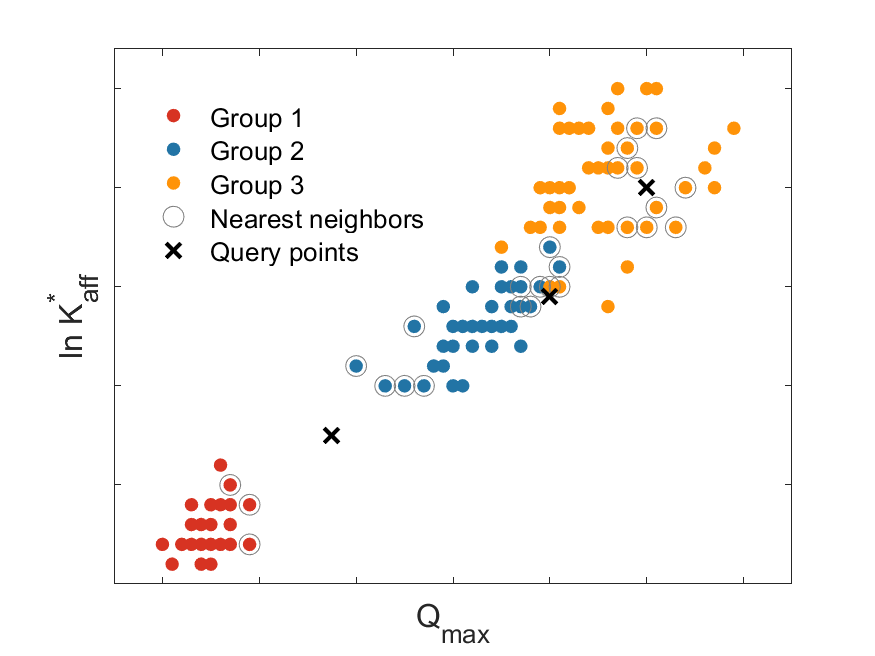
\includegraphics[width=0.75\linewidth]{KNN.png}
		\caption{$k$-Nearest Neighbours classification of adsorbent materials in the universal descriptor space $(Q_{\max},\, \ln K_{\mathrm{aff}}^{\ast})$. Three performance groups are shown: Group~1 (low capacity), Group~2 (intermediate), and Group~3 (high capacity). Query points ($\times$) are classified by majority vote among their $k = 10$ nearest neighbours (grey circles).\textbf{Note}: These is synthetic data to help understanding the classification model}
		\label{fig:KNN}
	\end{figure}

	% --- 5.5  Material classification: SVM ---
	\subsection{Material classification by Support Vector Machines}
	\label{sec:SVM}

	When the classification task requires a well-defined decision boundary, a Support Vector Machine (SVM) finds the maximum-margin separating hyperplane in descriptor space:
	\begin{equation}
		\min_{\mathbf{w},\,b}\;
		\frac{1}{2}\|\mathbf{w}\|^2
		+ C_{\mathrm{reg}}\sum_{i}\xi_i,
		\qquad
		y_i(\mathbf{w}\cdot\mathbf{x}_i + b) \ge 1 - \xi_i,
		\label{eq:SVM}
	\end{equation}
	where $\mathbf{w}$ is the normal to the hyperplane, $b$ is the bias, $\xi_i$ are slack variables for misclassified points, and $C_{\mathrm{reg}}$ controls the trade-off between margin width and classification error. The support vectors---the data points that lie on or within the margin---define the boundary entirely. Figure~\ref{fig:SVM}a shows a linear SVM separating two classes of adsorbents in the $(Q_{\max},\, \ln K_{\mathrm{aff}}^{\ast})$ plane (Eq.~\eqref{eq:Eads}).

	When the full universal descriptor set $\{Q_{\max},\, \ln K_{\mathrm{aff}}^{\ast},\, \sigma_H\}$ is used, the SVM operates in three dimensions and the decision boundary becomes a \emph{plane} (Figure~\ref{fig:SVM}b). For non-linearly separable data an RBF kernel $\mathcal{K}(\mathbf{x}_i, \mathbf{x}_j) = \exp(-\gamma\|\mathbf{x}_i - \mathbf{x}_j\|^2)$ replaces the linear kernel, producing curved decision surfaces that can capture complex group boundaries while still being defined entirely by the support vectors.

	\begin{figure}[H]
		\centering
		\begin{subfigure}[b]{0.48\linewidth}
			\centering
			\begin{overpic}[width=\linewidth]{SVM.png}
				\put(2,65){\textbf{(a)}}
			\end{overpic}
		\end{subfigure}
		\hfill
		\begin{subfigure}[b]{0.48\linewidth}
			\centering
			\begin{overpic}[width=\linewidth]{SVM_3D.png}
				\put(2,65){\textbf{(b)}}
			\end{overpic}
		\end{subfigure}
		\caption{Support Vector Machine classification of adsorbent materials. (a)~Two-dimensional projection onto the $(Q_{\max},\, \ln K_{\mathrm{aff}}^{\ast})$ plane: the solid line is the decision boundary $\mathbf{w}\!\cdot\!\mathbf{x} + b = 0$; dashed lines indicate the margin boundaries; support vectors are circled. (b)~Three-dimensional descriptor space $(Q_{\max},\, \ln K_{\mathrm{aff}}^{\ast},\, \sigma_H)$: decision boundaries are now planes (or curved surfaces when an RBF kernel is used). Three performance groups and two inter-group boundaries are shown; support vectors are marked with black circles. \textbf{Note}: These is synthetic data to help understanding the classification model}
		\label{fig:SVM}
	\end{figure}

	Categorical variables---such as material type (e.g.\ activated carbon, zeolite, MOF), best-fit isotherm model, or synthesis route---can be incorporated into the SVM framework through one-hot encoding. Each category is expanded into binary indicator features that enter $\mathbf{x}_i$ alongside the continuous descriptors $(Q_{\max},\, \ln K_{\mathrm{aff}}^{\ast},\, \sigma_H)$. In the resulting augmented feature space the SVM decision boundary is no longer a plane but a \emph{hyperplane} whose dimensionality equals the total number of features minus one. For a problem with $p$ continuous descriptors and $q$ one-hot columns the separating surface lives in $\mathbb{R}^{p+q}$ and its projection onto any two-dimensional descriptor pair produces the familiar boundary visualised in Figure~\ref{fig:SVM}a. Typical SVM classification tasks in adsorption studies include:
	\begin{itemize}
		\item \textbf{Binary screening:} suitable vs.\ unsuitable adsorbents for a given application (e.g.\ materials exceeding a regulatory removal threshold for drinking water).
		\item \textbf{Model-type separation:} distinguishing systems that are best described by a Langmuir-type isotherm ($\sigma_H \approx 0$) from those requiring a heterogeneous model (Sips, T\'{o}th).
		\item \textbf{Material-class boundaries:} separating material families (activated carbon vs.\ zeolite vs.\ MOF) in the descriptor space, using one-hot encoded material type as additional features.
		\item \textbf{Multi-class ranking:} extending the binary SVM via one-vs-one or one-vs-all strategies to classify adsorbents into three or more performance groups (as in Figure~\ref{fig:SVM}b).
	\end{itemize}

	Both KNN and SVM operate on the same standardised descriptor set (Eq.~\ref{SI-eq:si_standardise}) with Euclidean distance (Eq.~\ref{SI-eq:si_distance}). Ward's hierarchical clustering (Eq.~\ref{SI-eq:si_Ward}) provides an unsupervised alternative when class labels are unknown. The key advantage is that all three methods operate on model-independent quantities, ensuring that the grouping reflects intrinsic adsorption performance rather than artefacts of different fitting models. The full mathematical details of all clustering and classification methods are given in Section~\ref{SI-sec:si_clustering}.

	% =================================================================
	%  SECTION 6 — REPORTING GUIDELINES
	% =================================================================
	\section{Recommended reporting guidelines}
	\label{sec:guidelines}

	The following guidelines distill the preceding analysis into a practical reporting framework. Their goal is not to prescribe a single isotherm model but to ensure that, regardless of which model is selected, the published results are sufficient for cross-study comparison.

	% --- 6.1  Minimum reporting set ---
	\subsection{Minimum reporting set}
	\label{sec:min_reporting}

	For every adsorbent--adsorbate system analysed, the following quantities should be reported:
	\begin{enumerate}
		\item \textbf{Experimental conditions:} temperature $T$, pH, ionic strength, and the declared standard-state concentration $C^{0}$ (with units).
		\item \textbf{Model fit:} best-fit model name, all fitted parameters $\boldsymbol{\theta}$ with units and confidence intervals, and at least SSE, $R^2$, ARED, and AIC$_c$.
		\item \textbf{Universal descriptors:} $Q_{\max}$ (mg.g$^{-1}$), $K_{\mathrm{aff}}^{\ast}$ (dimensionless), $E_{\mathrm{ads}}$ (kJ\,mol$^{-1}$), and $\sigma_H$ (kJ\,mol$^{-1}$).
		\item \textbf{Comparison metrics} (when applicable): OVL between competing model distributions and/or cluster labels from KNN/SVM classification.
	\end{enumerate}
	The complete minimum reporting table is given in Table~\ref{SI-tab:si_reporting}; the extraction formulas for each model are collected in Table~\ref{SI-tab:si_extraction}.

	% --- 6.2  Analysis workflow ---
	\subsection{Recommended analysis workflow}
	\label{sec:workflow}

	We recommend a seven-step pipeline:
	\begin{enumerate}
		\item \textbf{Data collection.} Record $q_e$--$C_e$ pairs at constant $T$ and pH, with at least $n \geq 8$ points spanning the linear, transition, and plateau regions.
		\item \textbf{Non-linear fitting.} Fit all candidate models by non-linear least squares (Section~\ref{sec:fitting}).
		\item \textbf{Error metrics.} Compute SSE, $R^2$, $R^2_{\mathrm{adj}}$, ARED, and HYBRID for each model (Section~\ref{SI-sec:si_residuals}).
		\item \textbf{Model selection.} Rank by AIC$_c$; apply F-tests for nested pairs; apply physical decision criteria (Section~\ref{sec:Ftest}, Figure~\ref{SI-fig:si_decision_tree}).
		\item \textbf{Descriptor extraction.} From the selected model, compute $Q_{\max}$, $K_{\mathrm{aff}}^{\ast}$, $E_{\mathrm{ads}}$, and $\sigma_H$ (Table~\ref{tab:extraction}).
		\item \textbf{Statistical comparison.} Compute OVL between energy distributions of alternative models or between different materials (Section~\ref{SI-sec:si_OVL}).
		\item \textbf{Classification.} Map materials into the standardised descriptor space and apply clustering or supervised classification (Section~\ref{sec:KNN}, Section~\ref{sec:SVM}).
	\end{enumerate}

	% --- 6.3  Practical recommendations ---
	\subsection{Practical recommendations}
	\label{sec:practical}

	\begin{itemize}
		\item \textbf{Never linearise.} Linearised isotherm forms distort the error structure and bias the fitted parameters. Always use non-linear regression.
		\item \textbf{Do not report $Q_{\max}$ from the Freundlich equation.} The Freundlich isotherm has no saturation; any ``capacity'' derived from it is a concentration-window artefact.
		\item \textbf{Always declare $C^{0}$.} The numerical value of $E_{\mathrm{ads}}$ depends on $C^{0}$; omitting it renders the result non-reproducible. Differences $\Delta E_{\mathrm{ads}}$ between materials measured under the same $C^{0}$ are invariant.
		\item \textbf{Report confidence intervals.} Bootstrap or Monte Carlo uncertainties on $Q_{\max}$, $E_{\mathrm{ads}}$, and $\sigma_H$ should accompany every table entry.
		\item \textbf{Use $\sigma_H$ to assess model necessity.} If the best 3-parameter model yields only weak heterogeneity, e.g.\ $\sigma_H \leq RT$ or, for Sips, $m$ remains close to 1, the Langmuir model is likely sufficient and the extra parameter is not justified (Eq.~\ref{SI-eq:si_criterion_LvsS}).
		\item \textbf{Prefer the simplest adequate model.} Among models with $\Delta\mathrm{AIC}_c < 2$, report the one with the fewest parameters.
	\end{itemize}

	% =================================================================
	%  SECTION 7 — CONCLUSIONS
	% =================================================================
	\section{Conclusions}
	\label{sec:conclusions}

	% The current practice of tabulating $Q_{\max}$ and affinity constants from different isotherm models as though they were interchangeable is mathematically inconsistent and physically misleading. Units, asymptotic behavior, and the physical meaning of fitted parameters vary from model to model, making direct comparisons unreliable.

	% This work proposes a reporting framework that resolves the incompatibility through three measures. First, maximum capacity $Q_{\max}$ should be reported only from isotherm models that define a finite saturation plateau; the Freundlich equation, which lacks this feature, is unsuitable for capacity comparison. Second, raw affinity constants should be replaced by the standard-state adsorption energy $E_{\mathrm{ads}} = RT\ln K_{\mathrm{aff}}^{\ast}$, derived from a dimensionless equilibrium constant normalised by a declared standard-state concentration $C^{0}$. This places all models on a common thermodynamic scale. Third, the energy-distribution width $\sigma_E$ provides a universal measure of surface heterogeneity, enabling differentiation between homogeneous and heterogeneous surfaces regardless of the model chosen.

	% Together, the three descriptors $\{Q_{\max},\, E_{\mathrm{ads}},\, \sigma_E\}$ constitute a model-independent fingerprint for any adsorbent--adsorbate system. When combined with the model-selection pipeline described here---non-linear fitting, information criteria, F-tests, and physically motivated decision criteria---this framework provides a rigorous yet practical path from raw isotherm data to comparable, reproducible, and statistically validated descriptors.

	% The adoption of these guidelines would enable credible cross-study material screening, reliable benchmarking, and machine-learning classification of adsorption performance. As the contaminant landscape broadens to include PFAS, pharmaceuticals, and other emerging pollutants, such a common language is no longer optional---it is essential for rational sorbent development and for delivering on the promise of SDG~6.

	%%%%%%%%%%%%%%%%%%%%%%%%%%%%%%%%%%%%%%%%%%%%%%%%%%%%%%%%%%%%%%%%%%%%%
	\begin{acknowledgement}
		%TODO
	\end{acknowledgement}

	\begin{suppinfo}
		% Section~S-2: Isotherm model equations and limits for all 14 candidate models.
		% Section~S-3: Residual error metrics (SSE, $R^2$, $R^2_{\mathrm{adj}}$, EABS, RESID, ARED, MPSED, HYBRID) and information criteria (AIC, AIC$_c$, BIC, Akaike weights).
		% Section~S-4: Model-selection procedure---ranking, F-test, OVL, specific comparison criteria, and complete decision tree (Figure~S-\ref{SI-fig:si_decision_tree}).
		% Section~S-5: Energy distributions $f(E)$ for all isotherm models---general framework, summary tables, individual derivations, and figures.
		% Section~S-6: Clustering and classification methodology (feature standardisation, distance metric, KNN, SVM, Ward linkage).
		% Section~S-7: Complete reporting protocol---minimum reporting set and descriptor extraction tables.
	\end{suppinfo}

	\bibliography{references}
	
\end{document}
